\documentclass[11pt,a4paper]{article}
\usepackage[margin=2.15cm]{geometry}
\usepackage{fontspec}
\setmainfont{Arial}
\setsansfont{Arial}
\usepackage[spanish,es-nodecimaldot]{babel}
\usepackage{amsmath,amssymb}
\usepackage{graphicx}
\usepackage{booktabs,longtable,tabularx,array}
\usepackage{float}
\usepackage{xcolor}
\usepackage{hyperref}
\usepackage{fancyhdr}
\usepackage{enumitem}
\usepackage{caption}
\usepackage{microtype}

\definecolor{azul}{HTML}{174A6E}
\definecolor{azulclaro}{HTML}{EAF2F8}
\definecolor{gris}{HTML}{F4F6F7}
\hypersetup{
  colorlinks=true,
  linkcolor=azul,
  urlcolor=azul,
  citecolor=azul,
  pdftitle={Documento Final - Modelos de predicción DMI TerraBovina}
}
\pagestyle{fancy}
\fancyhf{}
\lhead{TerraBovina: predicción de DMI}
\rhead{Documento Final}
\cfoot{\thepage}
\setlength{\headheight}{14pt}
\setlength{\parindent}{0pt}
\setlength{\parskip}{5pt}
\setlist{nosep,leftmargin=1.4em}
\captionsetup{font=small,labelfont=bf}
\newcommand{\codigo}[1]{\nolinkurl{#1}}
\newcommand{\DMI}{\textit{DMI}}

\begin{document}

\begin{titlepage}
\centering
\vspace*{2.3cm}
{\Huge\bfseries Documento Final\par}
\vspace{0.7cm}
{\LARGE Predicción del consumo diario de materia seca en bovinos\par}
\vspace{0.35cm}
{\Large Modelo V1 Ridge y modelo V2 mejorado por especialistas\par}
\vfill
{\large Proyecto TerraBovina\par}
\vspace{0.3cm}
{\large Análisis del dataset, entrenamiento, validación, métricas y comparación\par}
\vfill
{\large Julio de 2026\par}
\end{titlepage}

\tableofcontents
\newpage

\section{Resumen ejecutivo}

Este trabajo desarrolla un sistema de aprendizaje automático para estimar el \textbf{consumo diario de materia seca} de bovinos. La variable estimada es \codigo{dmi_kg_dia}, expresada en kilogramos de materia seca por animal y por día. El propósito es obtener una aproximación cuantitativa a partir de información simple del animal: peso vivo, categoría, condición corporal y estado fisiológico.

El conjunto disponible contiene \textbf{3.833 observaciones}, \textbf{17 columnas}, \textbf{1.639 identificadores animales} y \textbf{131 hogares o fincas} de Bomet, Kenia. Como existen mediciones repetidas, los registros no son 3.833 animales independientes. La validación mantiene cada hogar enteramente en entrenamiento o prueba para reducir fuga de información.

Se presentan dos soluciones. El \textbf{modelo V1} es una regresión Ridge con $\alpha=10$, seleccionada entre cuatro candidatos mediante validación cruzada de cinco folds. Obtuvo MAE 1,1019, RMSE 1,5354 y $R^2=0,6821$. El \textbf{modelo V2 mejorado} es un \codigo{CategoryBlendRegressor}: conserva Ridge como base y utiliza especialistas diferentes según la categoría animal. Su evaluación anidada obtuvo MAE 1,0791, RMSE 1,5332 y $R^2=0,6830$.

Por resultados, la recomendación es V2 mejorado. Su ventaja global es realista pero pequeña: reduce el MAE aproximadamente 2,07\% respecto de V1. La mejora más clara aparece en Ternero/Ternera; Vaquilla empeora levemente y Toro presenta resultados mixtos. V1 continúa siendo una alternativa valiosa por simplicidad, transparencia y bajo costo de mantenimiento.

\section{Introducción}

\subsection{¿Por qué se realiza este trabajo?}

El consumo es una variable central para describir la relación entre un animal y su alimentación. Sin una estimación razonable del consumo resulta difícil comparar animales, analizar eficiencia, planificar recursos o construir herramientas de apoyo para sistemas ganaderos. Medir el consumo individual de forma directa puede requerir infraestructura, seguimiento y tiempo; por eso se estudia si puede aproximarse mediante variables disponibles con mayor facilidad.

El objetivo no es reemplazar una medición real ni formular automáticamente una dieta. Se busca construir una herramienta predictiva reproducible que aprenda asociaciones presentes en un conjunto histórico y estime un valor esperado para nuevos registros similares.

\subsection{Materia seca y DMI}

La materia seca es la parte del alimento que queda después de retirar el agua. Permite comparar alimentos con distinta humedad utilizando una base común. DMI proviene de \textit{Dry Matter Intake} y representa el consumo diario de materia seca.

Además del consumo absoluto, una predicción puede expresarse como porcentaje del peso vivo:
\begin{equation}
\text{DMI \% PV}=\frac{\widehat{\text{DMI}}\;(\text{kg/día})}{\text{peso vivo}\;(\text{kg})}\times100.
\end{equation}
Esta salida facilita comparar animales de tamaños diferentes. La columna histórica \codigo{dmi_pct_peso_vivo} no se utiliza como entrada porque se calcula a partir del objetivo real; incluirla permitiría al modelo conocer indirectamente la respuesta y produciría fuga de información.

\subsection{Objetivo general}

Construir y comparar modelos de regresión capaces de estimar \codigo{dmi_kg_dia}, manteniendo un proceso común de preparación, evitando compartir hogares entre entrenamiento y prueba, y evaluando el rendimiento global y por categoría.

\subsection{Objetivos específicos}
\begin{itemize}
  \item Comprender la estructura, contenido y limitaciones del dataset.
  \item Definir las variables que pueden utilizarse sin fuga de información.
  \item Entrenar una referencia estable e interpretable mediante Ridge.
  \item Desarrollar una solución mejorada con especialistas por categoría.
  \item Medir MAE, RMSE, $R^2$ y sesgo fuera de muestra.
  \item Comparar ambos modelos globalmente, por categoría y por fold.
  \item Conservar modelos serializados para inferencia reproducible.
\end{itemize}

\section{Dataset}

\subsection{Origen, dimensión y unidad observacional}

El archivo procesado analizado se encuentra en el directorio \codigo{data/processed}. Los metadatos del proyecto lo sitúan en Bomet, Kenia. El archivo actual tiene 3.833 filas y 17 columnas, distribuidas en cuatro periodos. Contiene 1.639 identificadores animales y 131 hogares.

La unidad observacional es una medición animal-periodo. Un mismo animal puede aparecer más de una vez: 2.194 filas corresponden a identificadores que ya habían aparecido previamente. Por lo tanto, la cantidad de filas no debe confundirse con la cantidad de individuos independientes.

El repositorio no conserva el CSV crudo original, una URL, licencia o hash de origen. El archivo procesado y los reportes disponibles son la fuente verificable del análisis. Algunas referencias históricas mencionan 3.840 filas y siete exclusiones; como esa transformación original no puede reconstruirse, este documento utiliza la cifra comprobable actual de 3.833 observaciones.

\subsection{Diccionario completo de las 17 columnas}

\small
\begin{longtable}{p{3.7cm}p{1.5cm}r p{7.8cm}}
\toprule
\textbf{Columna} & \textbf{Tipo} & \textbf{Nulos} & \textbf{Descripción y uso}\\
\midrule
\endhead
\codigo{animal_id} & texto & 0 & Identificador del animal o medición. Se conserva para identificar resultados, pero no entra al modelo.\\
\codigo{hh} & entero & 0 & Hogar o finca. Se utiliza como grupo de validación para evitar compartir hogares entre entrenamiento y prueba.\\
\codigo{kenya_category} & texto & 0 & Categoría original en inglés. Se conserva como referencia y no entra al modelo.\\
\codigo{categoria_terrabovina} & texto & 0 & Categoría normalizada: Vaca, Vaquilla, Novillo, Toro o Ternero/Ternera. Es una entrada categórica.\\
\codigo{periodo} & entero & 0 & Periodo de observación. No entra al modelo.\\
\codigo{periodo_fechas} & texto & 0 & Intervalo temporal expresado como texto. No entra al modelo.\\
\codigo{fecha_inicio} & texto & 291 & Fecha inicial de la observación. No entra al modelo.\\
\codigo{fecha_fin} & texto & 202 & Fecha final de la observación. No entra al modelo.\\
\codigo{peso_vivo_kg} & decimal & 0 & Peso vivo en kilogramos. Es la principal entrada numérica.\\
\codigo{condicion_corporal} & decimal & 2.111 & Condición corporal. Se utiliza para vacas; para las demás categorías se trata como ausente.\\
\codigo{dmi_kg_dia} & decimal & 0 & Variable objetivo: consumo diario de materia seca.\\
\codigo{dmi_pct_peso_vivo} & decimal & 0 & DMI como porcentaje del peso. Se excluye porque deriva del objetivo.\\
\codigo{outlier_peso} & booleano & 0 & Bandera de peso atípico. Todas las filas actuales están en falso.\\
\codigo{outlier_dmi_abs} & booleano & 0 & Bandera de DMI absoluto atípico. Todas las filas actuales están en falso.\\
\codigo{outlier_dmi_pct_bw} & booleano & 0 & Bandera de DMI relativo atípico. Todas las filas actuales están en falso.\\
\codigo{id_ambiguo} & booleano & 0 & Marca ambigüedad del identificador. Hay 1.421 filas marcadas; no se usa como predictor.\\
\codigo{estado_fisiologico_norm} & texto & 0 & Estado fisiológico normalizado. Es una entrada categórica, principalmente informativa para vacas.\\
\bottomrule
\end{longtable}
\normalsize

\subsection{Variables utilizadas}

Ambos modelos parten de las mismas cuatro entradas básicas:
\begin{itemize}
  \item \codigo{peso_vivo_kg};
  \item \codigo{categoria_terrabovina};
  \item \codigo{condicion_corporal};
  \item \codigo{estado_fisiologico_norm}.
\end{itemize}

La salida supervisada es \codigo{dmi_kg_dia}. El hogar \codigo{hh} no predice: solo controla las particiones. Identificadores, fechas, periodos, banderas y porcentaje de DMI quedan fuera de las entradas. Esta selección reduce fuga y mantiene un contrato sencillo para inferencia.

\subsection{Estadísticas principales}

\begin{table}[H]
\centering
\caption{Resumen de variables numéricas principales.}
\begin{tabular}{lrrrrr}
\toprule
\textbf{Variable} & \textbf{Media} & \textbf{Desv.} & \textbf{Mín.} & \textbf{Mediana} & \textbf{Máx.}\\
\midrule
Peso vivo (kg) & 203,4290 & 102,9078 & 19,6 & 208,3 & 595,5\\
Condición corporal & 2,6272 & 0,4249 & 1,5 & 2,5 & 4,5\\
DMI (kg/día) & 4,8285 & 2,7237 & 0,5862 & 4,2195 & 19,5070\\
DMI (\% peso vivo) & 2,5162 & 0,8284 & 0,5241 & 2,3724 & 5,9914\\
\bottomrule
\end{tabular}
\end{table}

La condición corporal tiene 2.111 ausencias, equivalentes aproximadamente al 55,1\% del dataset. Esto se relaciona con la regla de preparación que la conserva para vacas y la establece como ausente para las demás categorías. Los modelos no eliminan esas filas: utilizan imputación e indicadores de ausencia.

\subsection{Composición por categoría}

\begin{table}[H]
\centering
\caption{Composición y consumo por categoría.}
\resizebox{\textwidth}{!}{%
\begin{tabular}{lrrrrrrrr}
\toprule
\textbf{Categoría} & \textbf{Filas} & \textbf{Animales} & \textbf{Hogares} & \textbf{Peso medio} & \textbf{DMI medio} & \textbf{DMI mín.} & \textbf{Mediana} & \textbf{DMI máx.}\\
\midrule
Vaca & 1.722 & 604 & 129 & 280,168 & 6,6177 & 1,0384 & 6,1998 & 19,5070\\
Vaquilla & 777 & 370 & 95 & 175,358 & 3,9438 & 1,1710 & 3,6792 & 9,7778\\
Novillo & 282 & 155 & 61 & 140,246 & 3,6185 & 1,6809 & 3,4477 & 6,4448\\
Toro & 241 & 132 & 27 & 261,561 & 5,0970 & 1,9818 & 4,7054 & 12,6390\\
Ternero/Ternera & 811 & 378 & 123 & 72,078 & 2,2183 & 0,5862 & 2,0595 & 6,7181\\
\bottomrule
\end{tabular}}
\end{table}

Vaca es el grupo más numeroso, con mayor consumo medio y mayor dispersión. Toro y Novillo tienen menos observaciones y presencia en menos hogares, por lo que sus métricas son más sensibles a la composición de cada fold.

\subsection{Estado fisiológico}

Los valores presentes son DESCONOCIDO (2.112), L (992), P (330), N (201), B (190), P/L (5), B/L (2) y N/P (1). El código de ingeniería agrupa L, P/L y B/L como señales de lactancia; P, P/L y N/P como señales de preñez; y B y B/L como señales de estado seco. Estas interpretaciones pertenecen a la implementación del proyecto y deben validarse contra el diccionario original de la fuente antes de realizar conclusiones biológicas.

Los estados combinados tienen entre una y cinco observaciones. No existe información suficiente para estimar efectos propios estables de esos niveles.

\begin{figure}[H]
\centering
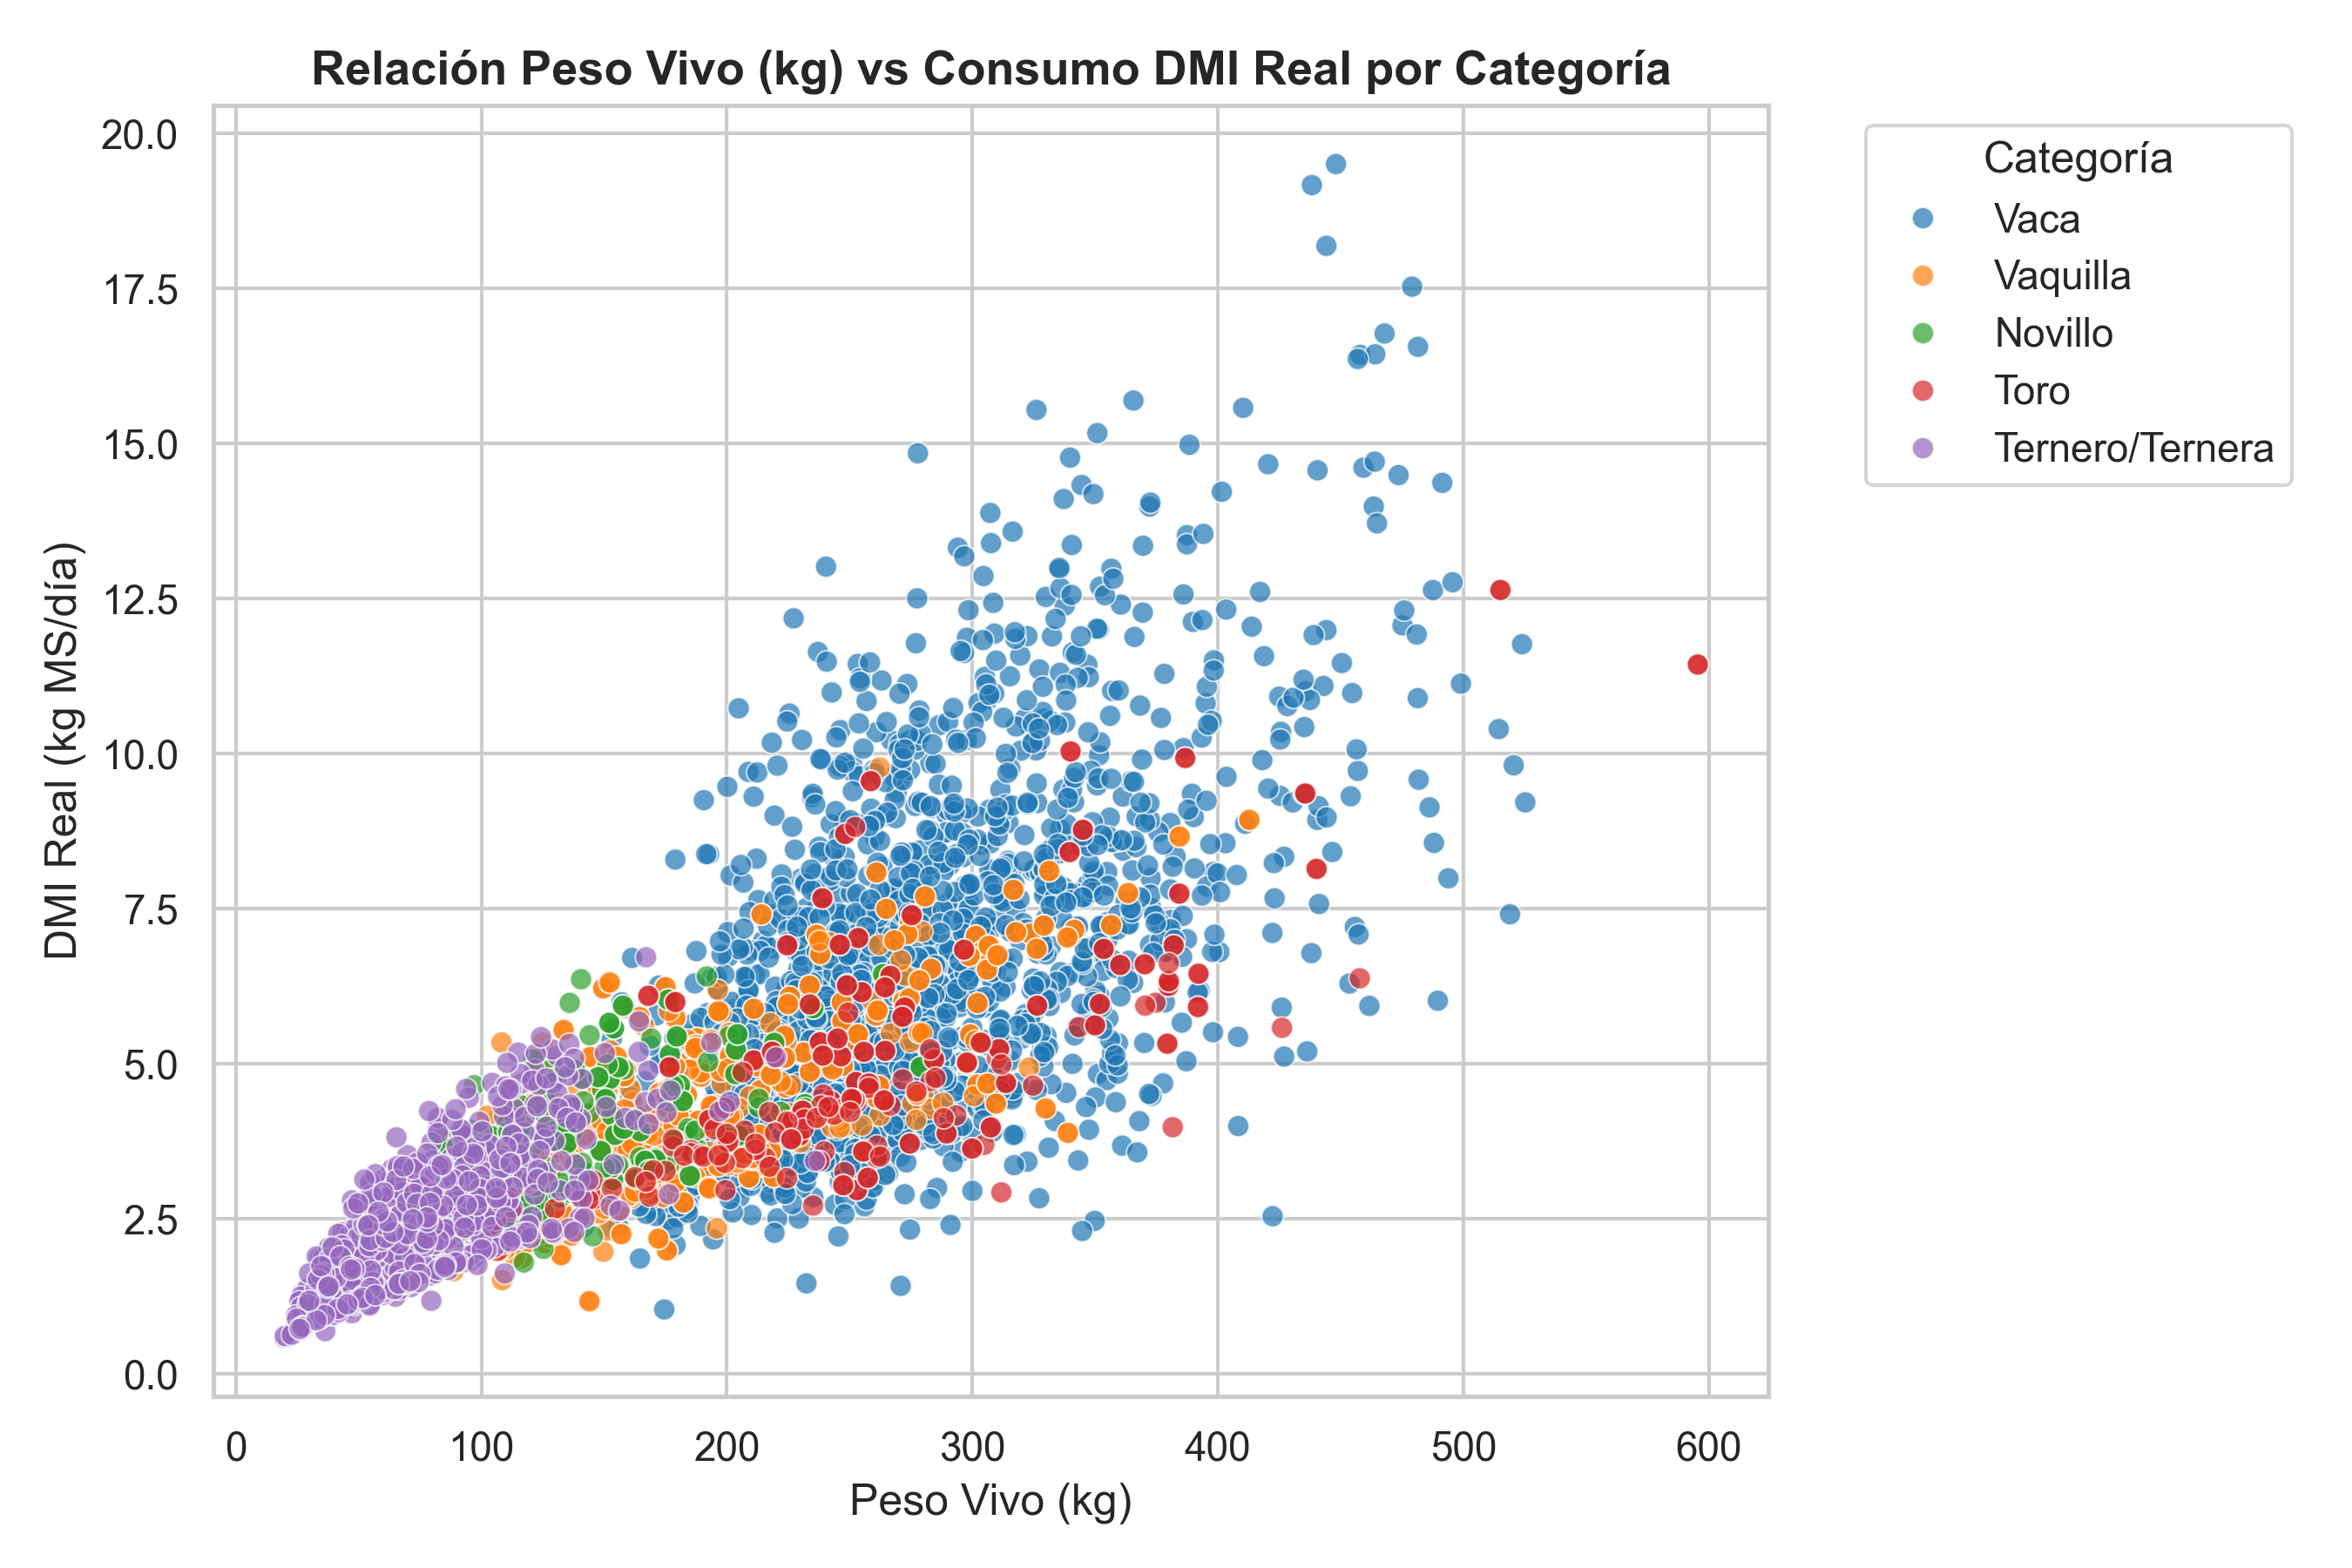
\includegraphics[width=0.91\textwidth]{figures/6_weight_vs_dmi_scatter.png}
\caption{Peso vivo frente a DMI observado. La asociación positiva explica por qué el peso aporta gran parte de la señal predictiva.}
\end{figure}

\begin{figure}[H]
\centering
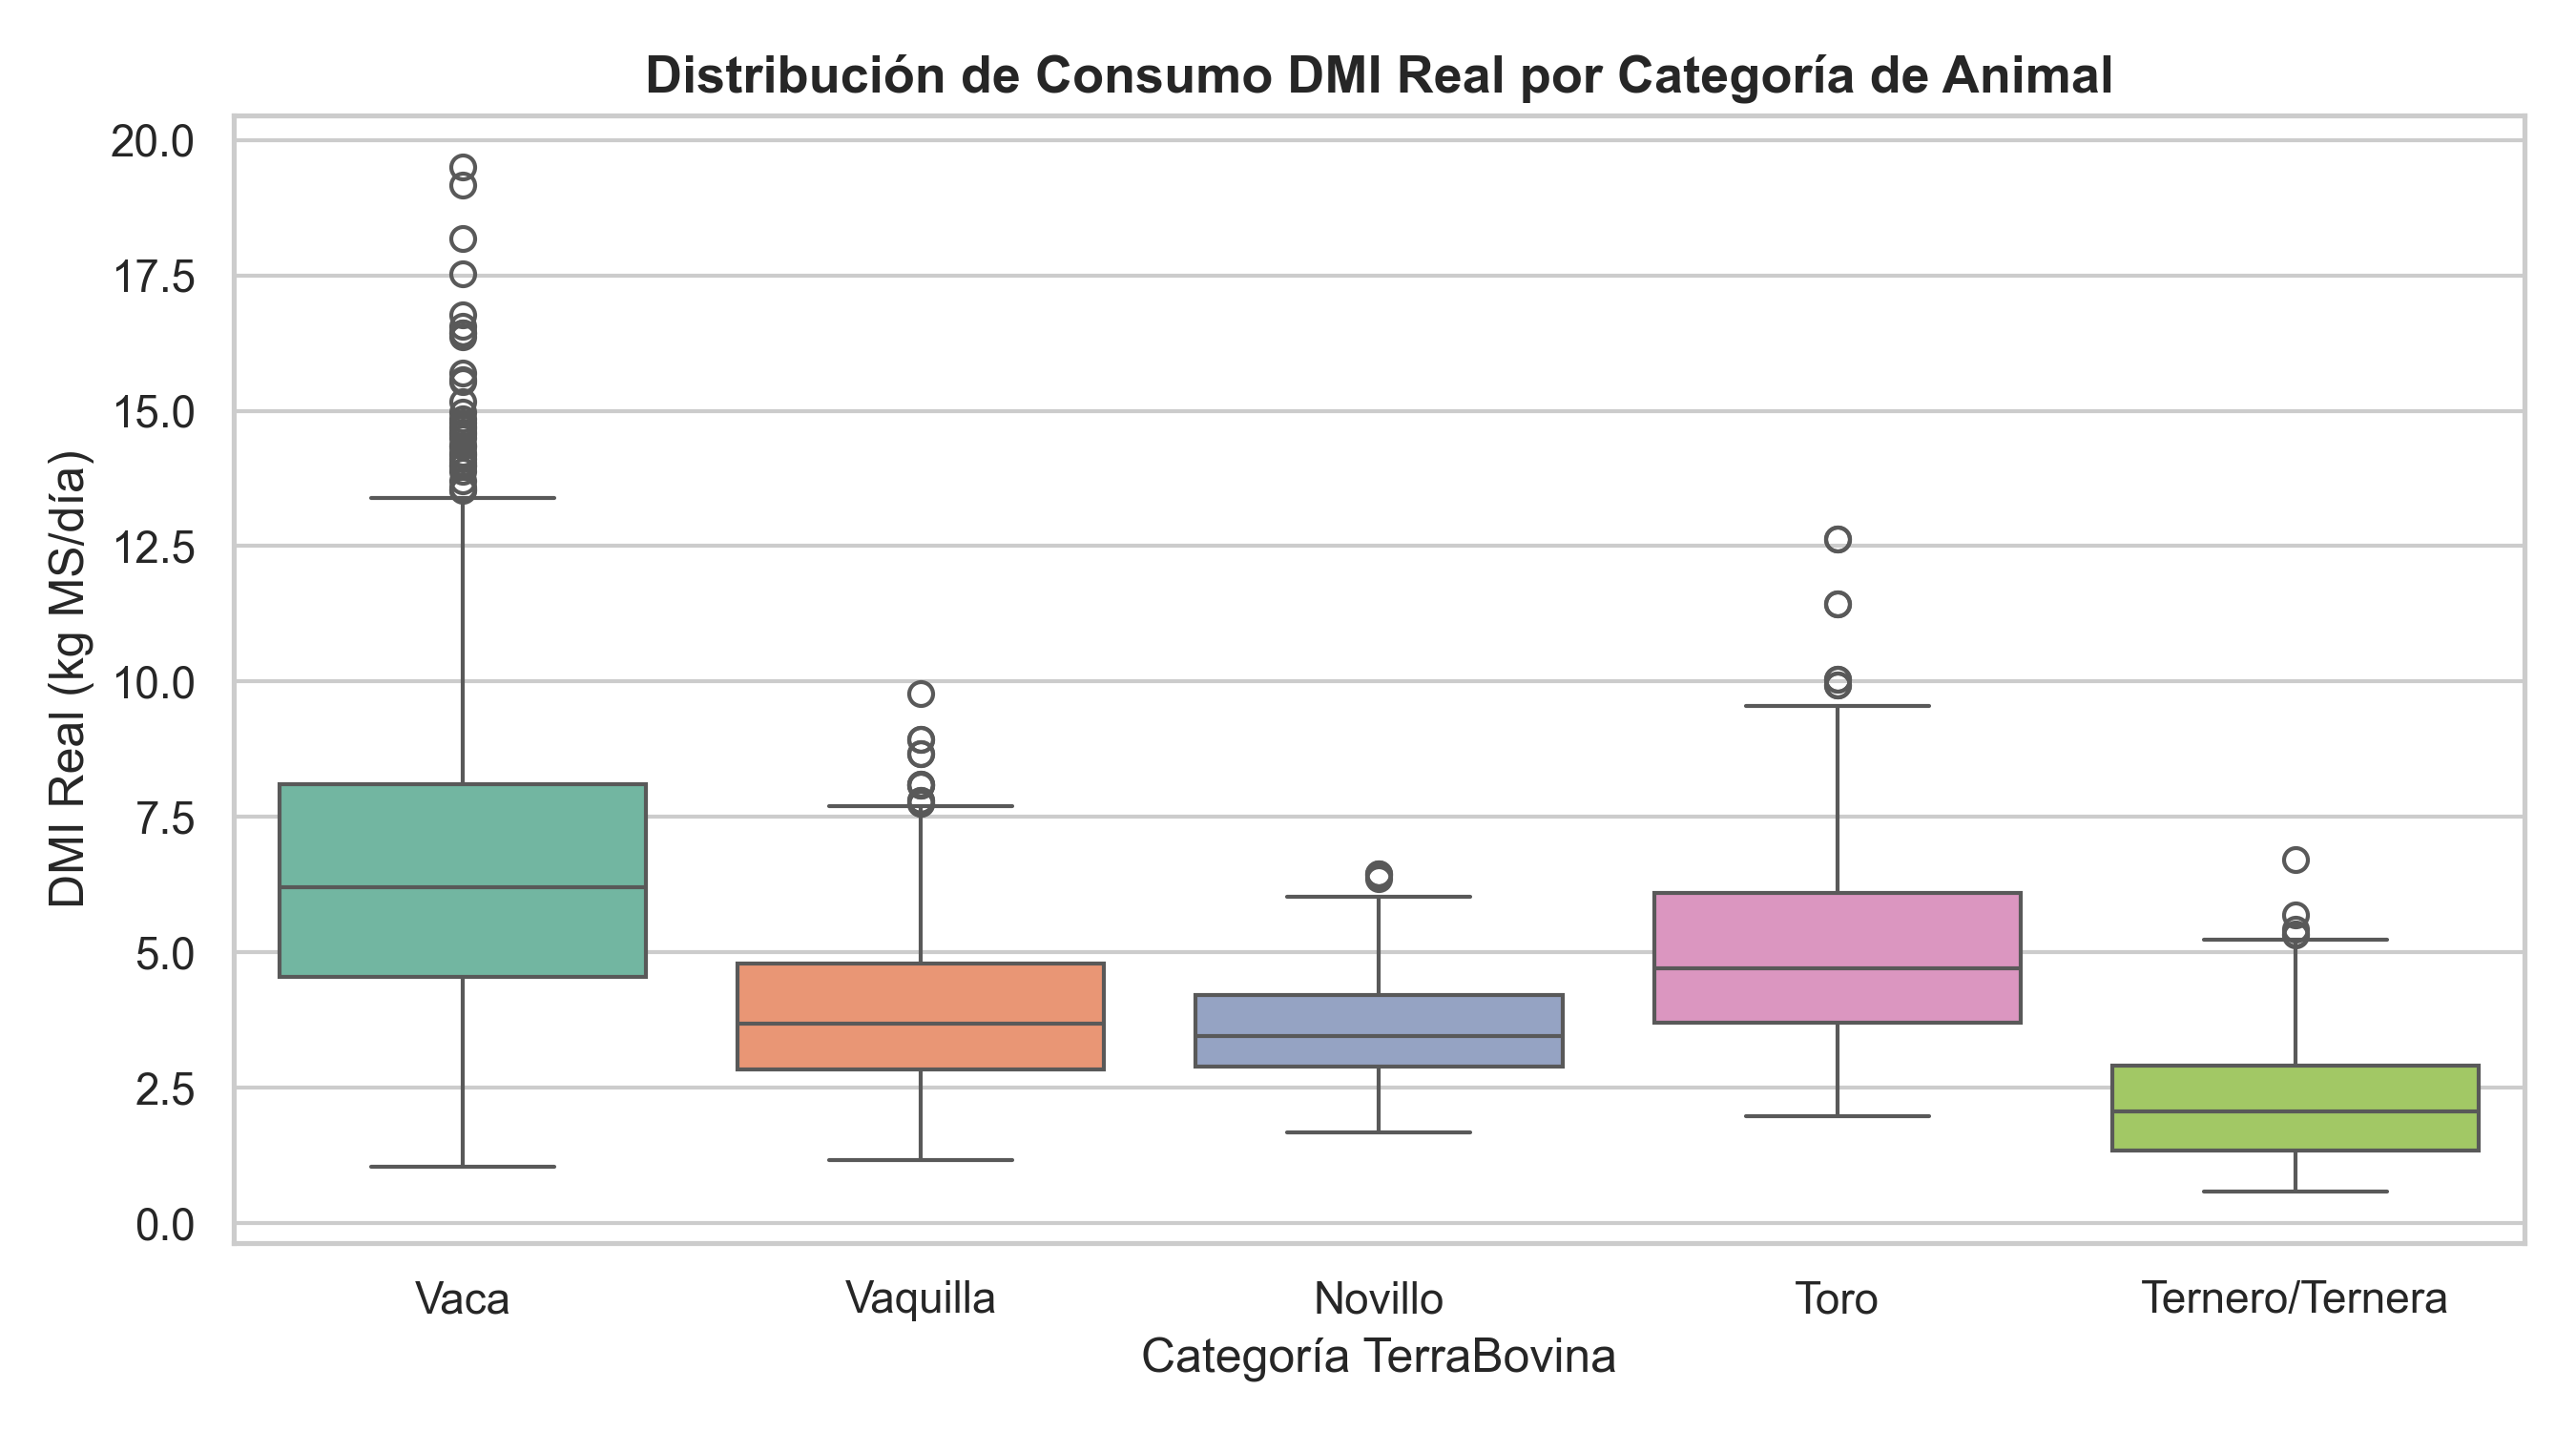
\includegraphics[width=0.91\textwidth]{figures/7_dmi_by_category_boxplot.png}
\caption{Distribución del DMI por categoría. Vaca presenta el rango y la variabilidad más altos.}
\end{figure}

\begin{figure}[H]
\centering
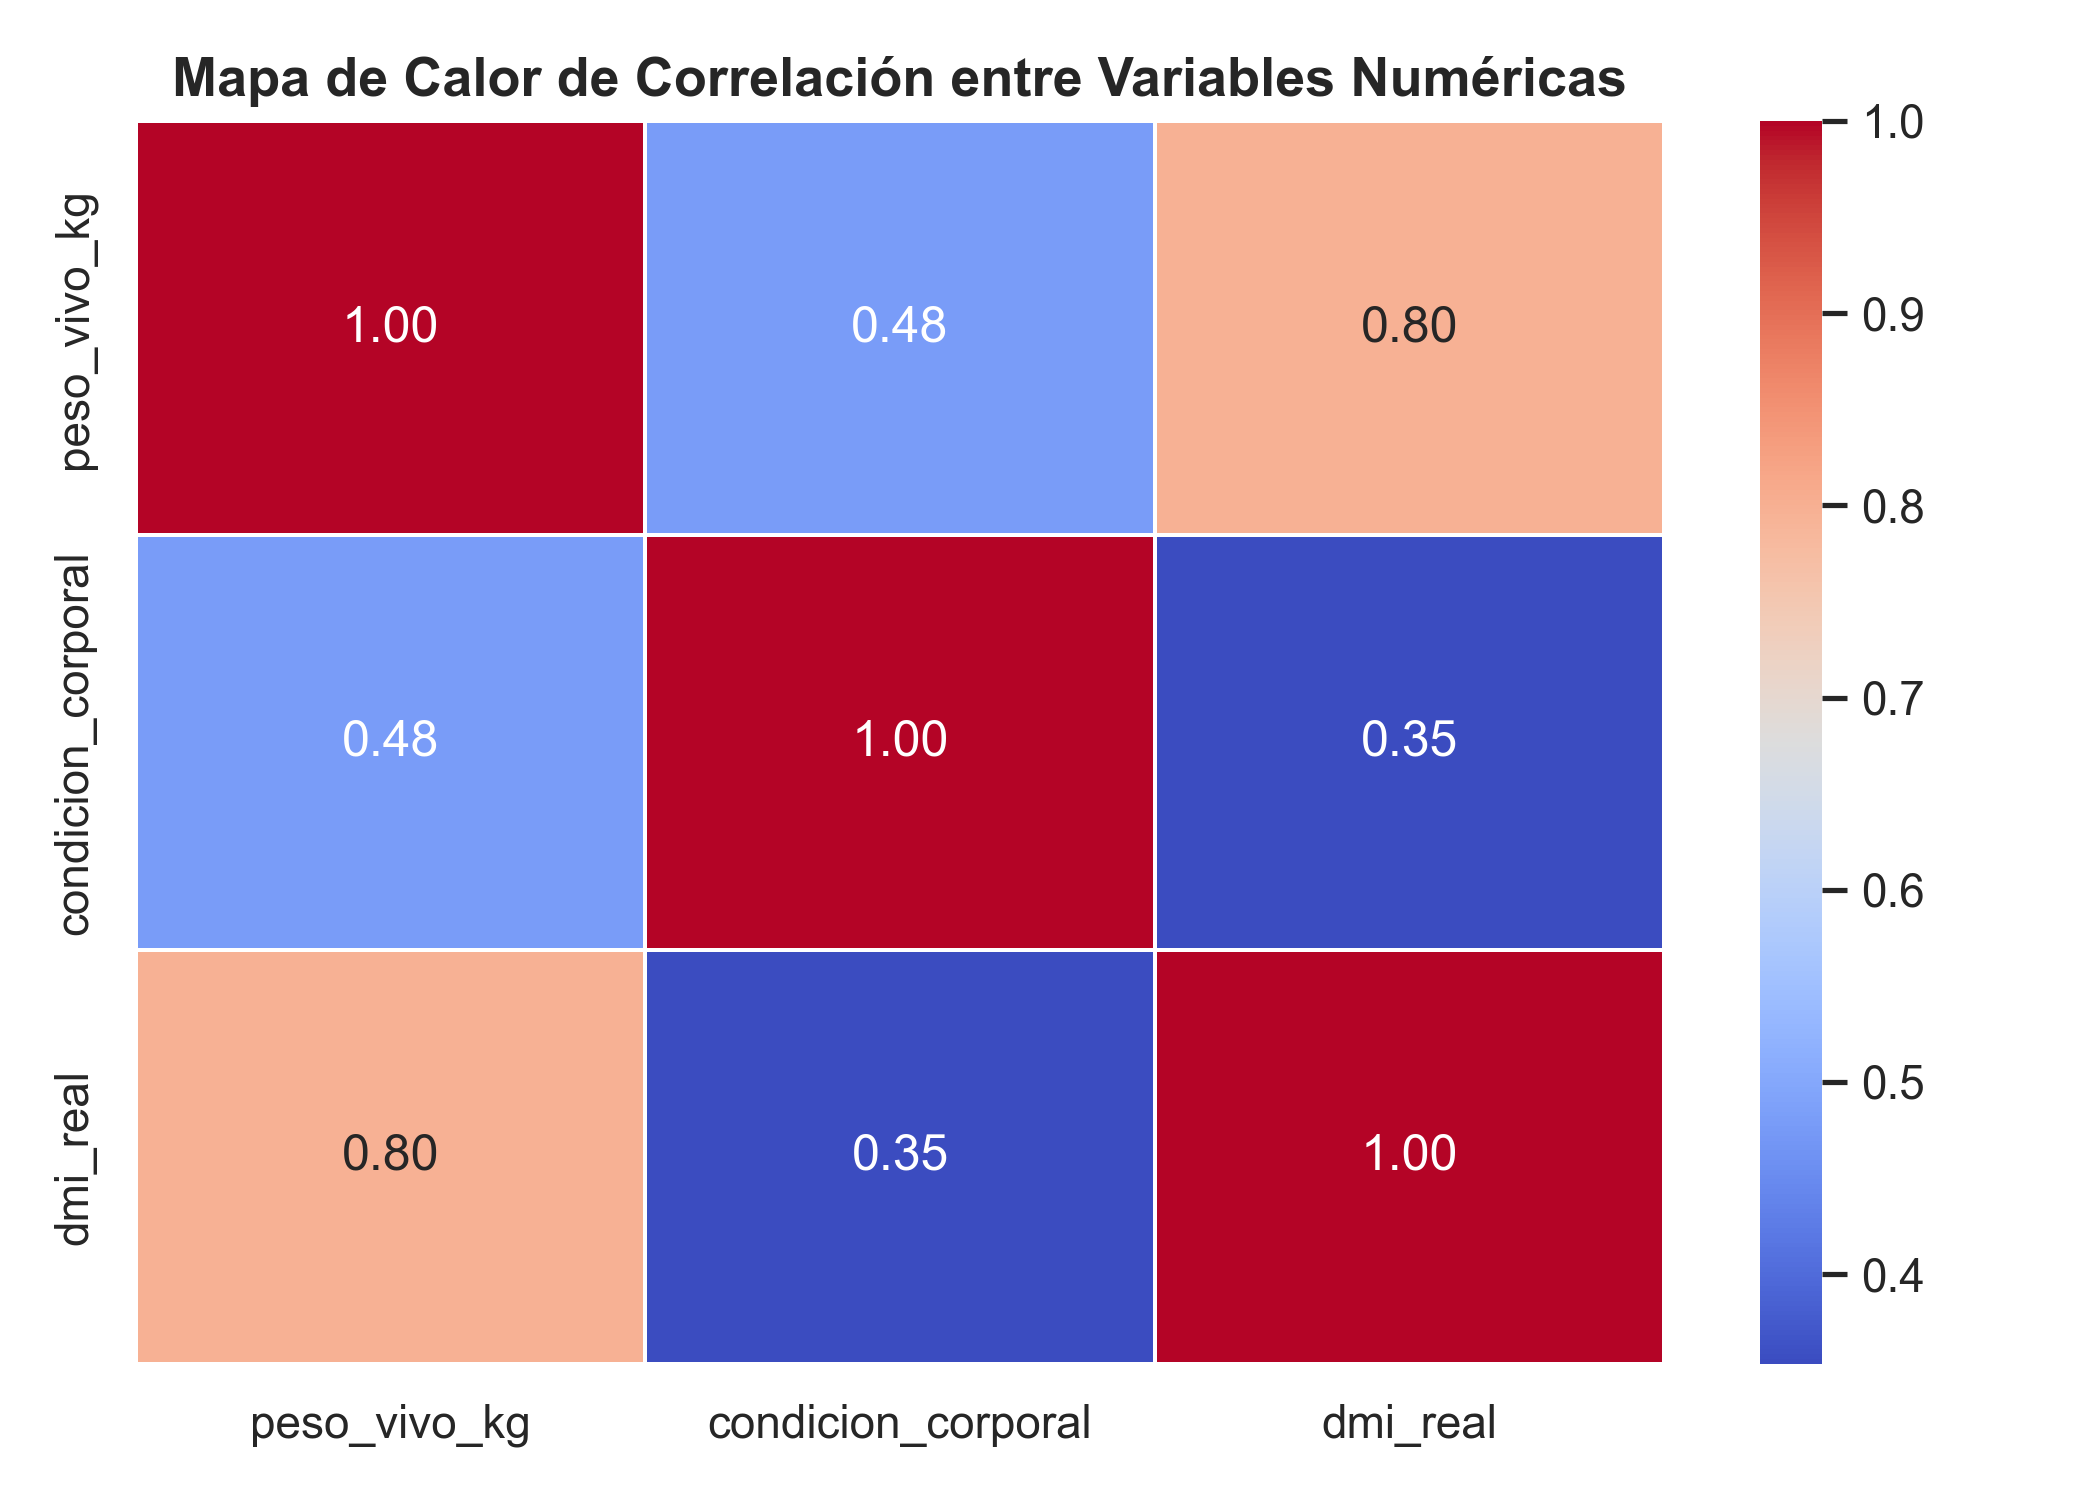
\includegraphics[width=0.72\textwidth]{figures/8_correlation_heatmap.png}
\caption{Correlaciones lineales de variables numéricas. Una asociación no implica causalidad ni representa todas las relaciones no lineales.}
\end{figure}

\section{Preparación común y metodología de evaluación}

\subsection{Preparación de entradas}

La función compartida de características verifica columnas, convierte peso y condición corporal a formato numérico y normaliza textos. Para categorías diferentes de Vaca fuerza \codigo{condicion_corporal} a ausente y \codigo{estado_fisiologico_norm} a DESCONOCIDO. Aplicar la misma función al entrenar y predecir evita discrepancias entre ambos momentos.

\subsection{Separación por hogares}

La evaluación utiliza \codigo{StratifiedGroupKFold}. La estratificación intenta conservar las proporciones de categorías y el agrupamiento obliga a que todas las filas de un hogar permanezcan en un solo lado de cada partición. Esto evita que el modelo se pruebe con observaciones del mismo establecimiento que utilizó para ajustarse.

Cada fila recibe una predicción \textit{out-of-fold}: el modelo que la predice no fue entrenado con su fold. Después se truncan resultados negativos a cero porque un consumo físico no puede ser negativo.

\subsection{Métricas y su Interpretación Práctica}

Para evaluar los modelos se utilizan cuatro métricas complementarias. Para cada observación $i$, el error de predicción se define como $e_i = y_i - \hat{y}_i$.

\textbf{1. MAE (Error Absoluto Medio) — Métrica Principal}
\begin{equation}
MAE = \frac{1}{n}\sum_{i=1}^{n}|y_i - \hat{y}_i|
\end{equation}
\begin{itemize}
  \item \textbf{¿Qué mide?} Se expresa directamente en kg MS/día. Representa, en términos prácticos, \textbf{por cuántos kilos se equivoca el modelo en promedio} por cada animal al día.
  \item \textbf{Interpretación:} Si el MAE global del modelo V2 es de $1,08\text{ kg}$, significa que ante una predicción de consumo de $5,0\text{ kg MS/día}$, el consumo real esperado del animal se ubicará típicamente entre $3,92$ y $6,08\text{ kg MS/día}$.
\end{itemize}

\textbf{2. Coeficiente de Determinación ($R^2$) — Capacidad Explicativa}
\begin{equation}
R^2 = 1 - \frac{\sum_i(y_i - \hat{y}_i)^2}{\sum_i(y_i - \bar{y})^2}
\end{equation}
\begin{itemize}
  \item \textbf{¿Qué mide?} Mide el \textbf{porcentaje de la variabilidad biológica que el modelo logra explicar} en comparación con un modelo trivial que solo responde el valor medio.
  \item \textbf{Interpretación:} Un $R^2$ de $0,683$ ($68,3\%$) significa que las variables de entrada (peso vivo, categoría ganadera y estado fisiológico) explican casi el $70\%$ de las diferencias de consumo entre animales. El $31,7\%$ restante se debe a factores no registrados en el dataset (clima, calidad nutricional del pasto, genética individual, entre otros).
\end{itemize}

\textbf{3. Error Relativo Porcentual ($\text{MAE} / \overline{\text{DMI}}$)}
\begin{itemize}
  \item \textbf{¿Qué mide?} El porcentaje de desviación respecto al consumo real promedio ($\overline{\text{DMI}} = 4,85\text{ kg MS/día}$).
  \item \textbf{Interpretación:} Evalúa el impacto del error según el tamaño y consumo del animal. Por ejemplo, en Novillos y Vaquillas el error relativo es inferior al $20\%$ ($18,2\%$ y $19,3\%$ respectivamente), lo cual constituye una precisión alta para modelos predictivos biológicos en producción ganadera.
\end{itemize}

\textbf{4. RMSE (Raíz del Error Cuadrático Medio)}
\begin{equation}
RMSE = \sqrt{\frac{1}{n}\sum_{i=1}^{n}(y_i - \hat{y}_i)^2}
\end{equation}
Se expresa en kg MS/día. A diferencia del MAE, penaliza cuadráticamente las desviaciones grandes, permitiendo detectar si existen errores atípicos significativos.

\textbf{5. Sesgo Medio}
\begin{equation}
\text{sesgo} = \frac{1}{n}\sum_i(y_i - \hat{y}_i)
\end{equation}
Mide la tendencia del modelo a subestimar ($\text{sesgo} > 0$) o sobreestimar ($\text{sesgo} < 0$) el consumo global. Un valor cercano a cero ($0,079\text{ kg}$) confirma la neutralidad de las predicciones.

\section{Modelo V1: regresión Ridge}

\subsection{Motivación y formulación}

V1 busca una solución estable, compacta e interpretable. Ridge es una regresión lineal regularizada que minimiza errores cuadrados y penaliza coeficientes grandes:
\begin{equation}
\min_{\beta_0,\boldsymbol{\beta}}
\sum_{i=1}^{n}(y_i-\beta_0-\mathbf{x}_i^T\boldsymbol{\beta})^2
+\alpha\sum_{j=1}^{p}\beta_j^2.
\end{equation}

Se utiliza $\alpha=10$. La penalización L2 contrae los coeficientes y reduce sensibilidad al ruido y a la colinealidad, sin llevarlos necesariamente a cero. La principal limitación es que representa relaciones mayormente lineales y aditivas.

\subsection{Pipeline de preprocesamiento}

Antes de ajustar Ridge se ejecutan los siguientes pasos:
\begin{enumerate}
  \item Imputación por mediana de peso y condición corporal.
  \item Creación de indicadores que señalan valores ausentes.
  \item Estandarización numérica con \codigo{StandardScaler}.
  \item Codificación one-hot de categoría y estado fisiológico.
  \item Configuración \codigo{handle_unknown="ignore"} para tolerar niveles no vistos.
\end{enumerate}

La estandarización aplica aproximadamente $z=(x-\mu)/\sigma$. Es importante porque Ridge debe penalizar coeficientes de variables que estén en escalas comparables.

\subsection{Candidatos y entrenamiento}

El entrenamiento original comparó cuatro configuraciones:
\begin{table}[H]
\centering
\caption{Candidatos evaluados para seleccionar V1.}
\begin{tabularx}{\textwidth}{p{3.2cm}X}
\toprule
\textbf{Candidato} & \textbf{Configuración y propósito}\\
\midrule
Baseline de la media & \codigo{DummyRegressor(strategy="mean")}; referencia mínima sin aprendizaje de relaciones.\\
Ridge & Regresión regularizada con $\alpha=10$.\\
Random Forest & 100 árboles, profundidad máxima 10 y semilla 42.\\
CatBoost & 500 iteraciones, profundidad 6, tasa 0,04, pérdida RMSE y semilla 42.\\
\bottomrule
\end{tabularx}
\end{table}

Se aplicaron cinco folds agrupados por hogar. Cada candidato produjo predicciones fuera de fold sobre todas las filas. La regla de selección fue el menor MAE global. Ridge ganó y luego se reentrenó sobre las 3.833 observaciones para crear \codigo{models/dmi_model.joblib}. Las métricas de generalización son las de validación, no las del ajuste final.

\subsection{Resultados de selección}

\begin{table}[H]
\centering
\caption{Resultados fuera de fold de los candidatos de V1.}
\begin{tabular}{lrrr}
\toprule
\textbf{Modelo} & \textbf{MAE} & \textbf{RMSE} & \textbf{$R^2$}\\
\midrule
Baseline media & 2,1280 & 2,7273 & -0,0029\\
\textbf{Ridge} & \textbf{1,1019} & \textbf{1,5354} & \textbf{0,6821}\\
Random Forest & 1,1611 & 1,6458 & 0,6348\\
CatBoost & 1,1027 & 1,5587 & 0,6724\\
\bottomrule
\end{tabular}
\end{table}

Ridge reduce el MAE del baseline aproximadamente 48,2\%. CatBoost queda prácticamente empatado en MAE, pero Ridge también obtiene mejor RMSE y $R^2$ en esta comparación. La diferencia pequeña frente a CatBoost no permite afirmar superioridad universal; solo justifica la selección bajo la regla implementada.

\begin{figure}[H]
\centering
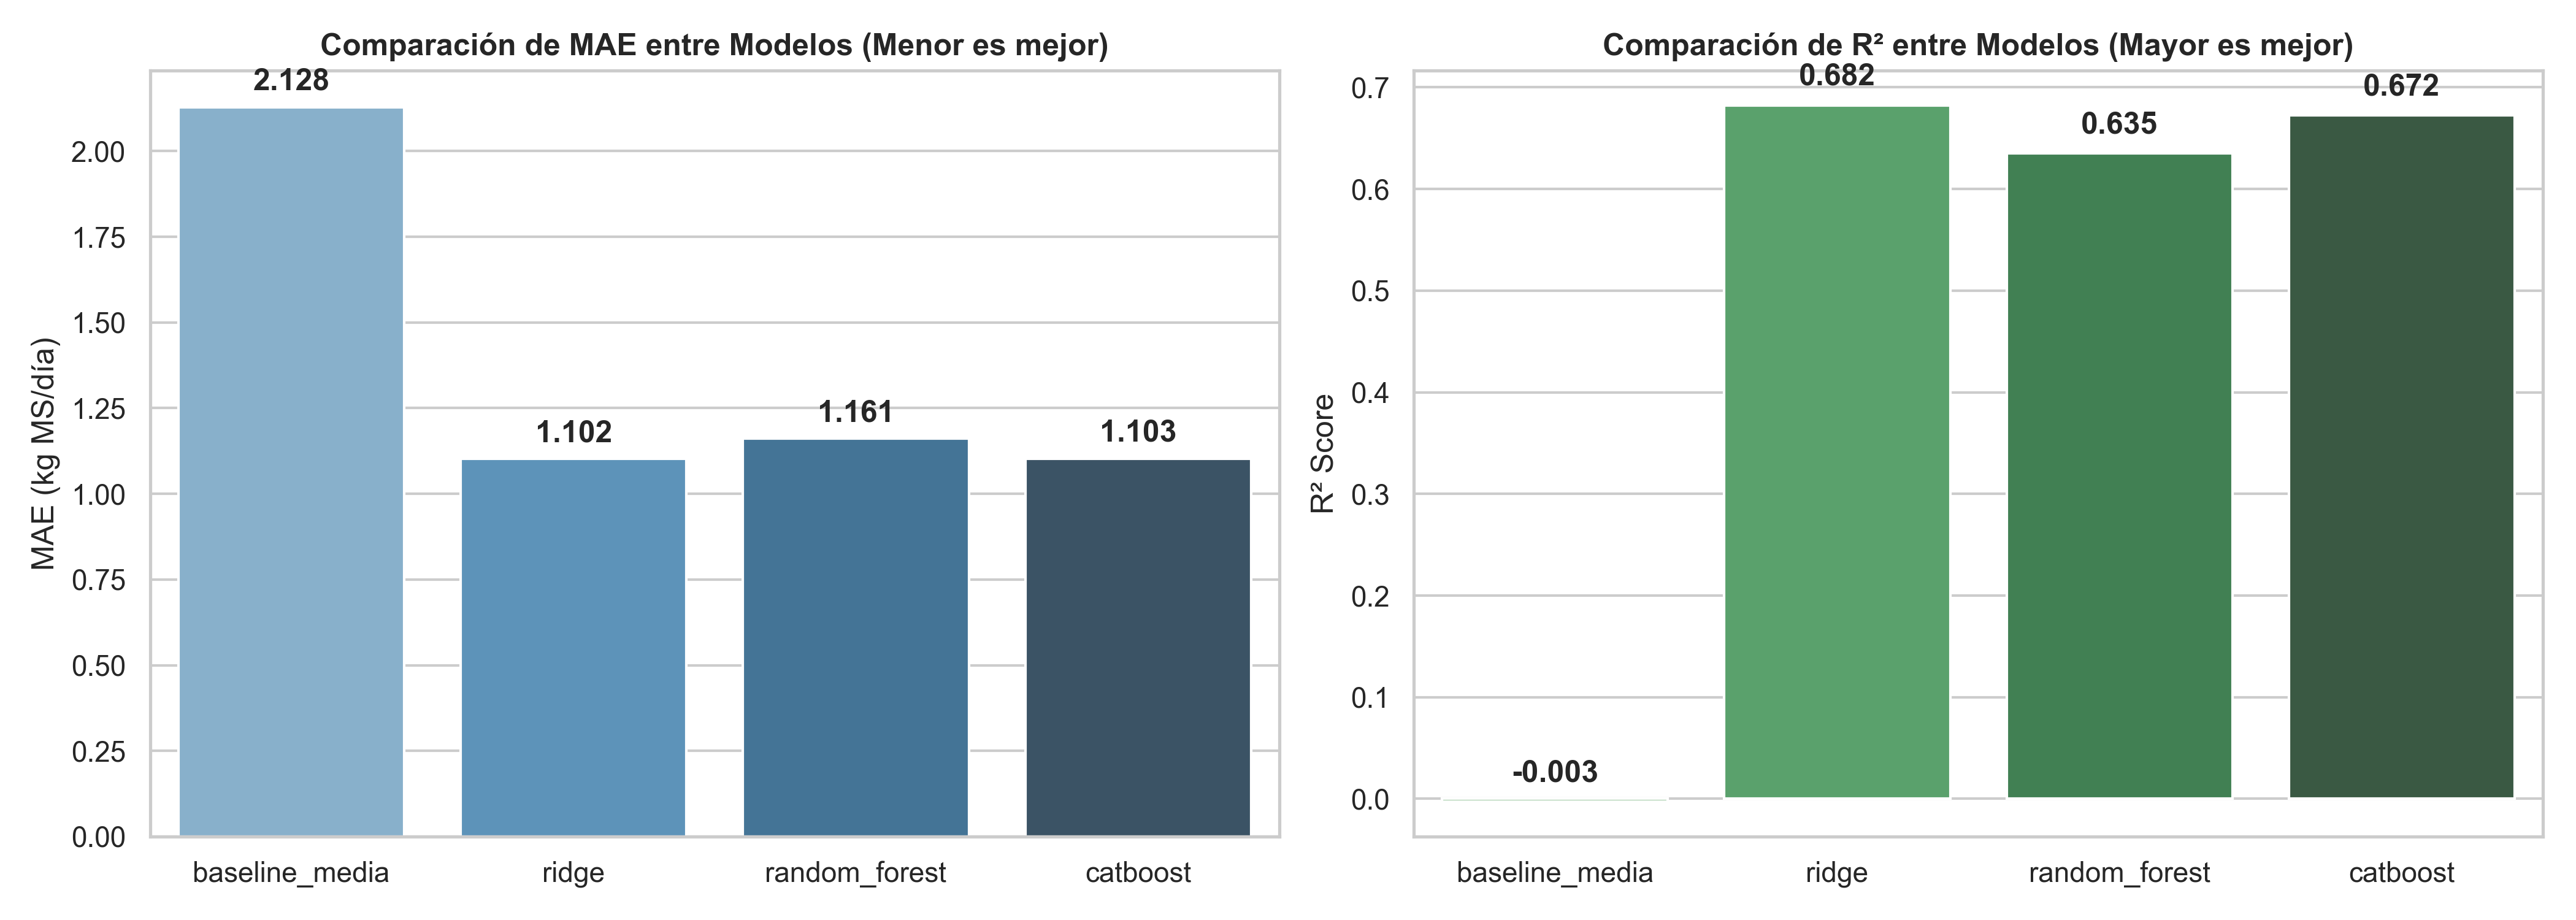
\includegraphics[width=\textwidth]{figures/1_model_comparison_mae_r2.png}
\caption{Comparación de candidatos durante el desarrollo de V1. Ridge fue el ganador formal.}
\end{figure}

\subsection{Estabilidad por fold}

\begin{table}[H]
\centering
\caption{Métricas de Ridge en los cinco folds.}
\begin{tabular}{crrr}
\toprule
\textbf{Fold} & \textbf{MAE} & \textbf{RMSE} & \textbf{$R^2$}\\
\midrule
1 & 1,1138 & 1,5369 & 0,6617\\
2 & 1,0993 & 1,5368 & 0,7214\\
3 & 1,1558 & 1,6039 & 0,6830\\
4 & 1,0742 & 1,4878 & 0,6818\\
5 & 1,0715 & 1,5164 & 0,6314\\
\bottomrule
\end{tabular}
\end{table}

El MAE varía entre 1,0715 y 1,1558. La oscilación es moderada, aunque cinco particiones no reemplazan intervalos de confianza ni validación externa.

\subsection{Métricas por categoría}

\begin{table}[H]
\centering
\caption{Resultados de Ridge V1 por categoría.}
\begin{tabular}{lrrr}
\toprule
\textbf{Categoría} & \textbf{MAE} & \textbf{RMSE} & \textbf{$R^2$}\\
\midrule
Vaca & 1,5857 & 2,0608 & 0,4110\\
Vaquilla & 0,7540 & 0,9449 & 0,6037\\
Novillo & 0,6639 & 0,8028 & 0,4126\\
Toro & 1,0204 & 1,3642 & 0,5068\\
Ternero/Ternera & 0,5846 & 0,7018 & 0,5858\\
\bottomrule
\end{tabular}
\end{table}

Vaca presenta el MAE más alto, coherente con su mayor nivel y dispersión de consumo. Esto no significa automáticamente que sea el peor grupo en términos relativos; una diferencia de escala produce errores absolutos mayores.

\subsection{Lectura de métricas: qué significan y qué tan buenas son}

Para expresar MAE y RMSE como porcentajes se los compara con el DMI medio del dataset, que es 4,8285 kg MS/día. Este porcentaje facilita dimensionar el error, pero no reemplaza las unidades originales ni constituye una regla universal de calidad.

\begin{table}[H]
\centering
\caption{Lectura práctica de las métricas globales de V1 Ridge.}
\begin{tabularx}{\textwidth}{p{2.5cm}p{2.8cm}X}
\toprule
\textbf{Métrica} & \textbf{Lectura porcentual} & \textbf{Interpretación}\\
\midrule
MAE 1,1019 & 22,82\% del DMI medio & Una predicción se desvía en promedio unos 1,10 kg MS/día. En términos de escala, el error típico equivale aproximadamente a 23 de cada 100 unidades del consumo medio.\\
RMSE 1,5354 & 31,80\% del DMI medio & Los errores grandes elevan la raíz cuadrática hasta 1,54 kg MS/día. Que supere al MAE indica que existe una cola de casos más difíciles.\\
$R^2=0,6821$ & 68,21\% de la variabilidad representada & El modelo captura una proporción importante de las diferencias observadas de consumo. No significa que acierte el 68,21\% de los animales.\\
MAE frente al baseline & Reducción de 48,22\% & V1 casi reduce a la mitad el error absoluto de predecir siempre la media, lo que demuestra que las variables aportan señal predictiva útil.\\
\bottomrule
\end{tabularx}
\end{table}

\subsubsection{Lectura por categoría}

Para comparar categorías con consumos de distinta escala, el MAE y el RMSE de cada grupo se dividen por su propio DMI medio. Un porcentaje menor indica un error pequeño respecto del consumo habitual de esa categoría. El $R^2$ se lee por separado: puede ser moderado aun cuando el error relativo sea bajo si el consumo del grupo varía dentro de un rango estrecho.

\begin{table}[H]
\centering
\caption{Lectura relativa de V1 Ridge por categoría.}
\resizebox{\textwidth}{!}{%
\begin{tabular}{lrrrrl}
\toprule
\textbf{Categoría} & \textbf{DMI medio} & \textbf{MAE relativo} & \textbf{RMSE relativo} & \textbf{$R^2$} & \textbf{Valoración}\\
\midrule
Vaca & 6,6177 & 23,96\% & 31,14\% & 41,10\% & Moderada; categoría difícil y dispersa.\\
Vaquilla & 3,9438 & 19,12\% & 23,96\% & 60,37\% & Buena; equilibrio favorable entre error y variabilidad.\\
Novillo & 3,6185 & 18,35\% & 22,19\% & 41,26\% & Buen error relativo; $R^2$ moderado.\\
Toro & 5,0970 & 20,02\% & 26,76\% & 50,68\% & Razonable, con margen de mejora.\\
Ternero/Ternera & 2,2183 & 26,35\% & 31,64\% & 58,58\% & Aceptable; error absoluto bajo pero relativo alto.\\
\bottomrule
\end{tabular}}
\end{table}

\begin{itemize}
  \item \textbf{Vaca:} el MAE de 1,5857 kg parece alto y también representa casi una cuarta parte de su consumo medio. El $R^2$ de 41,10\% indica capacidad moderada para distinguir consumos dentro del grupo. Es la categoría más exigente por su amplitud y dispersión.
  \item \textbf{Vaquilla:} el error típico equivale al 19,12\% del consumo medio y el modelo representa 60,37\% de la variabilidad. Es una de las lecturas más favorables de V1.
  \item \textbf{Novillo:} presenta el menor MAE relativo, 18,35\%, pero el $R^2$ es 41,26\%. El modelo se equivoca poco respecto de la escala media, aunque explica de forma moderada las diferencias entre novillos.
  \item \textbf{Toro:} el MAE relativo es 20,02\% y el $R^2$ 50,68\%. El rendimiento es razonable, pero el grupo tiene pocas observaciones y hogares, por lo que la estimación es menos estable.
  \item \textbf{Ternero/Ternera:} el MAE absoluto de 0,5846 kg es el menor, pero equivale al 26,35\% de su consumo medio. Es una demostración de por qué no debe evaluarse una categoría únicamente con kilogramos de error.
\end{itemize}

\textbf{¿Qué tan bueno es V1?} Su rendimiento puede calificarse como \textbf{bueno y útil como modelo predictivo interno}: supera ampliamente al baseline, explica cerca de dos tercios de la variabilidad y mantiene un comportamiento razonablemente estable entre folds. No debe calificarse como excelente ni como una medición precisa para cada animal, porque todavía deja aproximadamente 31,79\% de la variabilidad sin representar y su error típico ronda el 22,82\% del consumo medio.

No existe un umbral universal que convierta automáticamente un MAE en ``bueno'' o ``malo''. La valoración depende de la escala del consumo, del costo práctico de equivocarse, de la comparación con una referencia y de la población donde se use. Con estos datos, V1 es una base sólida; para decisiones nutricionales reales todavía requiere validación externa y local.

\begin{figure}[H]
\centering
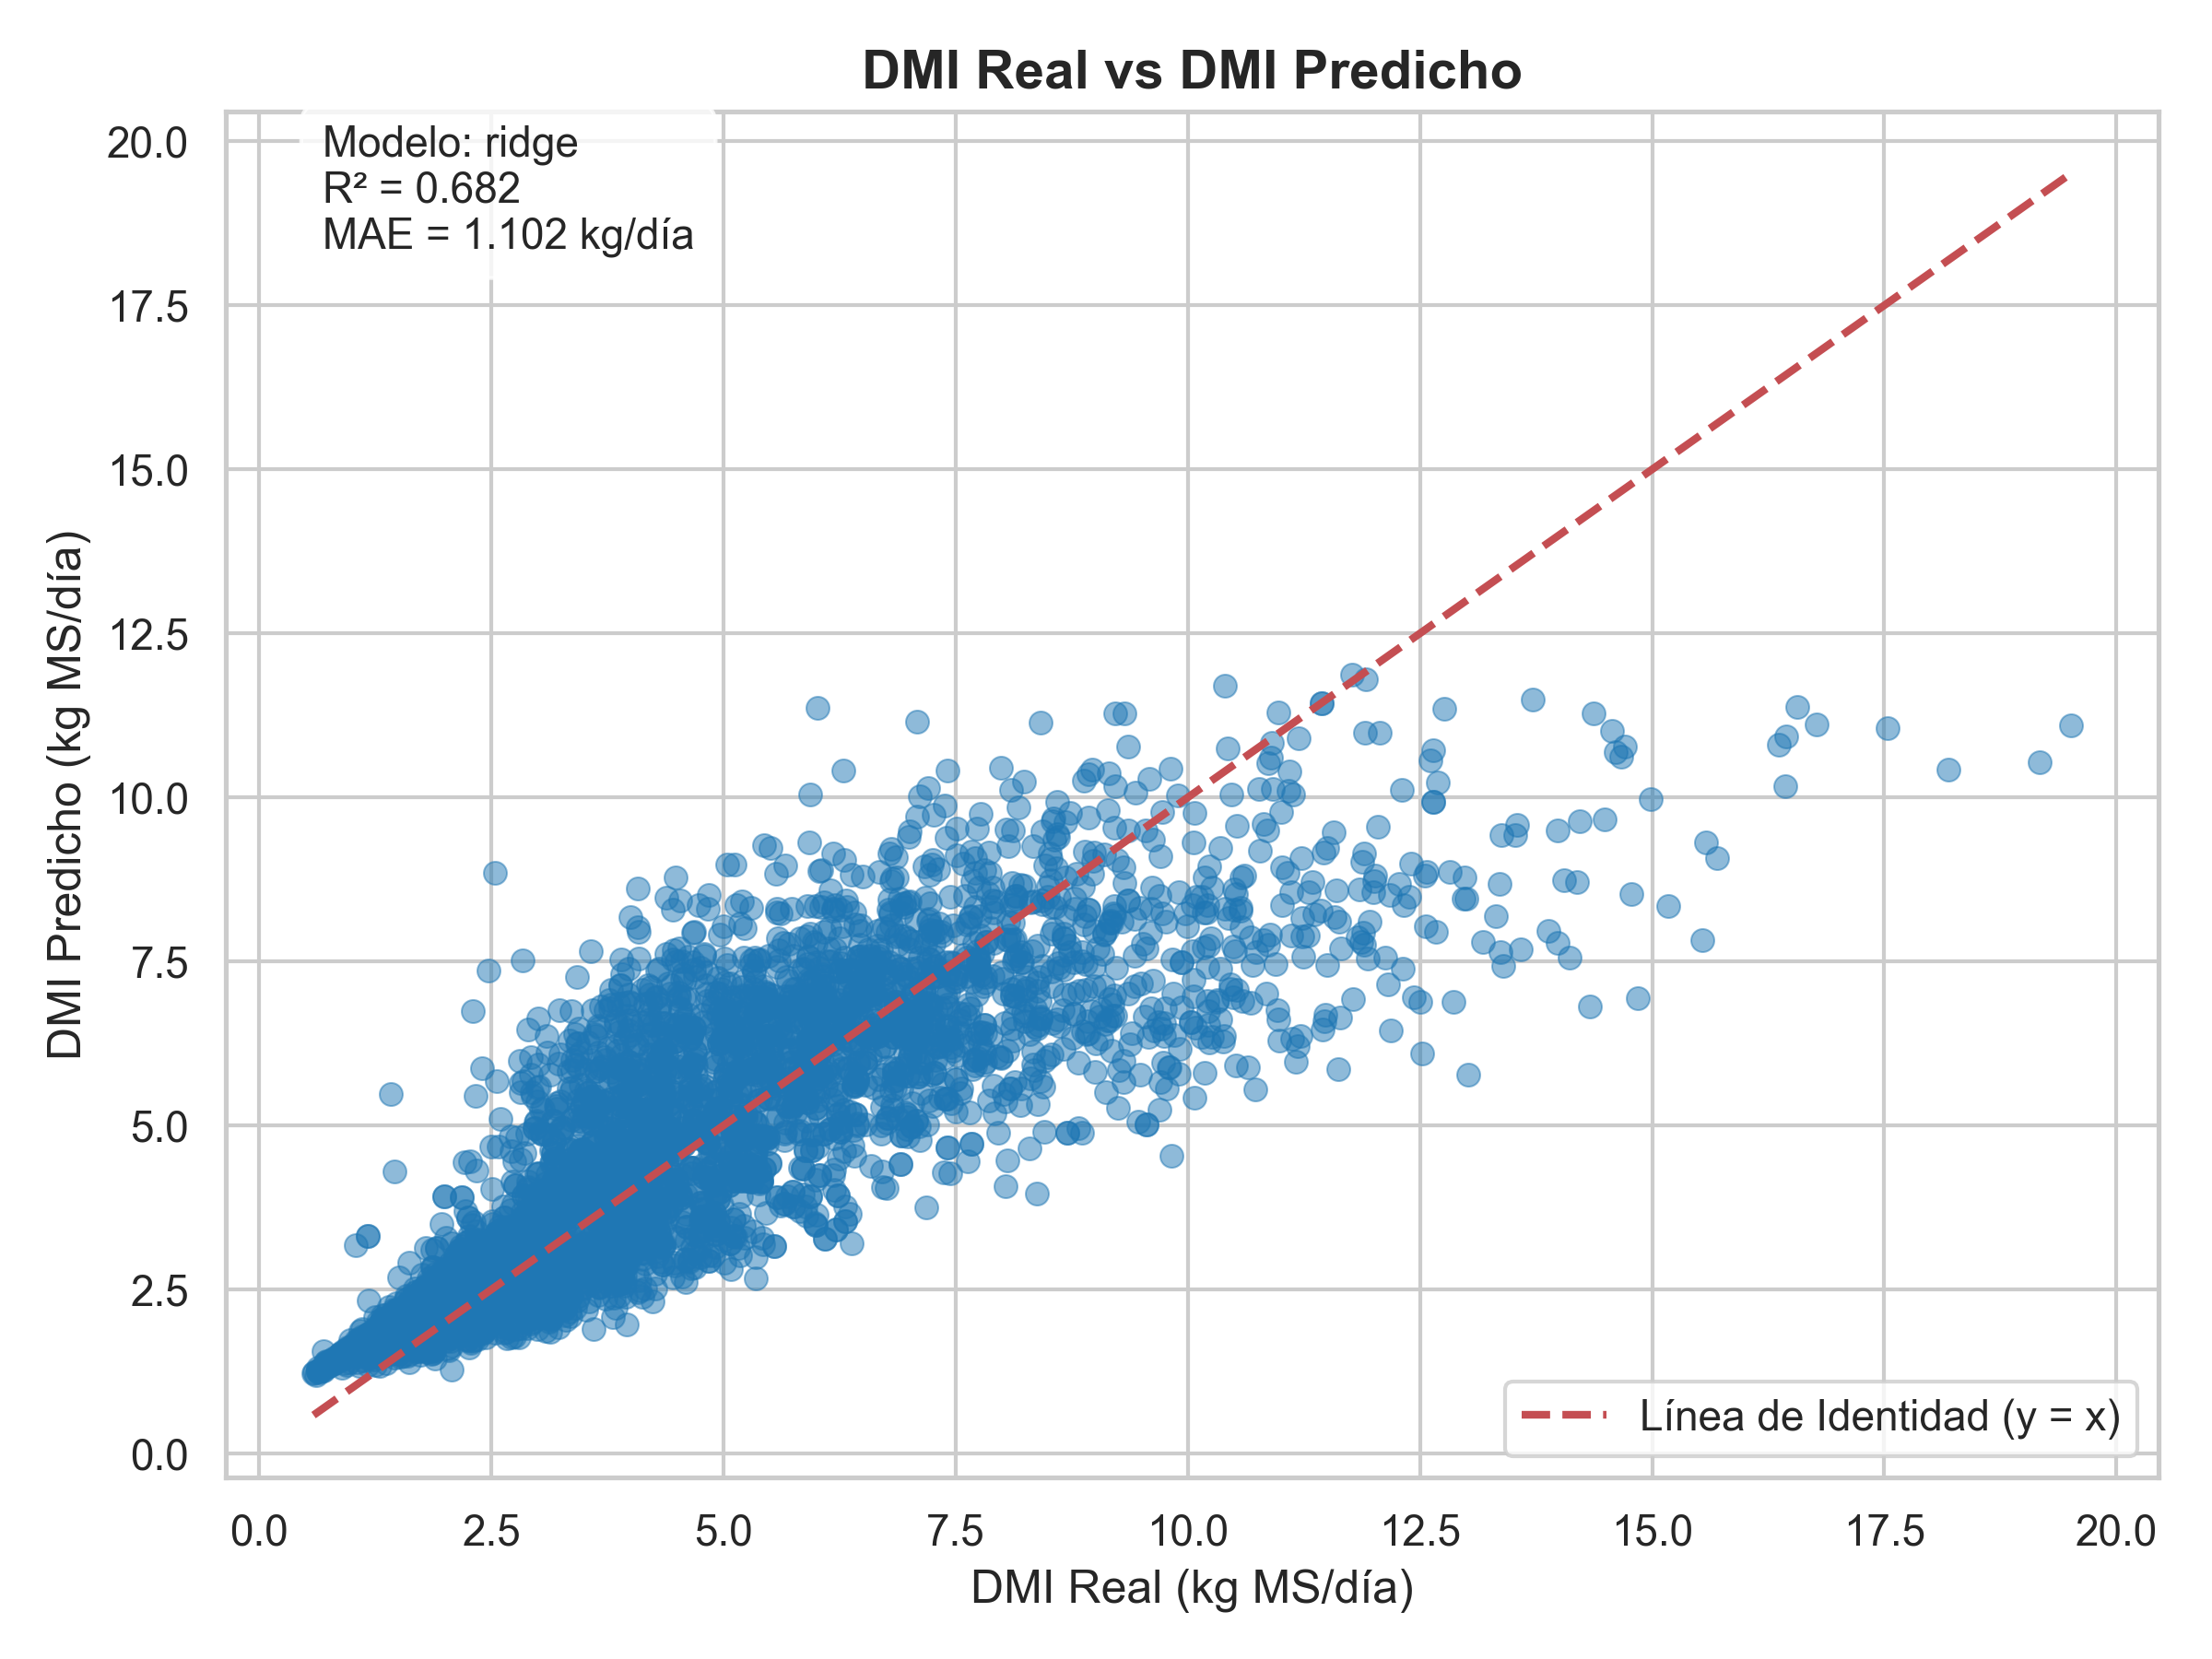
\includegraphics[width=0.84\textwidth]{figures/2_actual_vs_predicted.png}
\caption{DMI real frente a predicciones fuera de fold de Ridge V1. La diagonal representa predicción perfecta.}
\end{figure}

\begin{figure}[H]
\centering
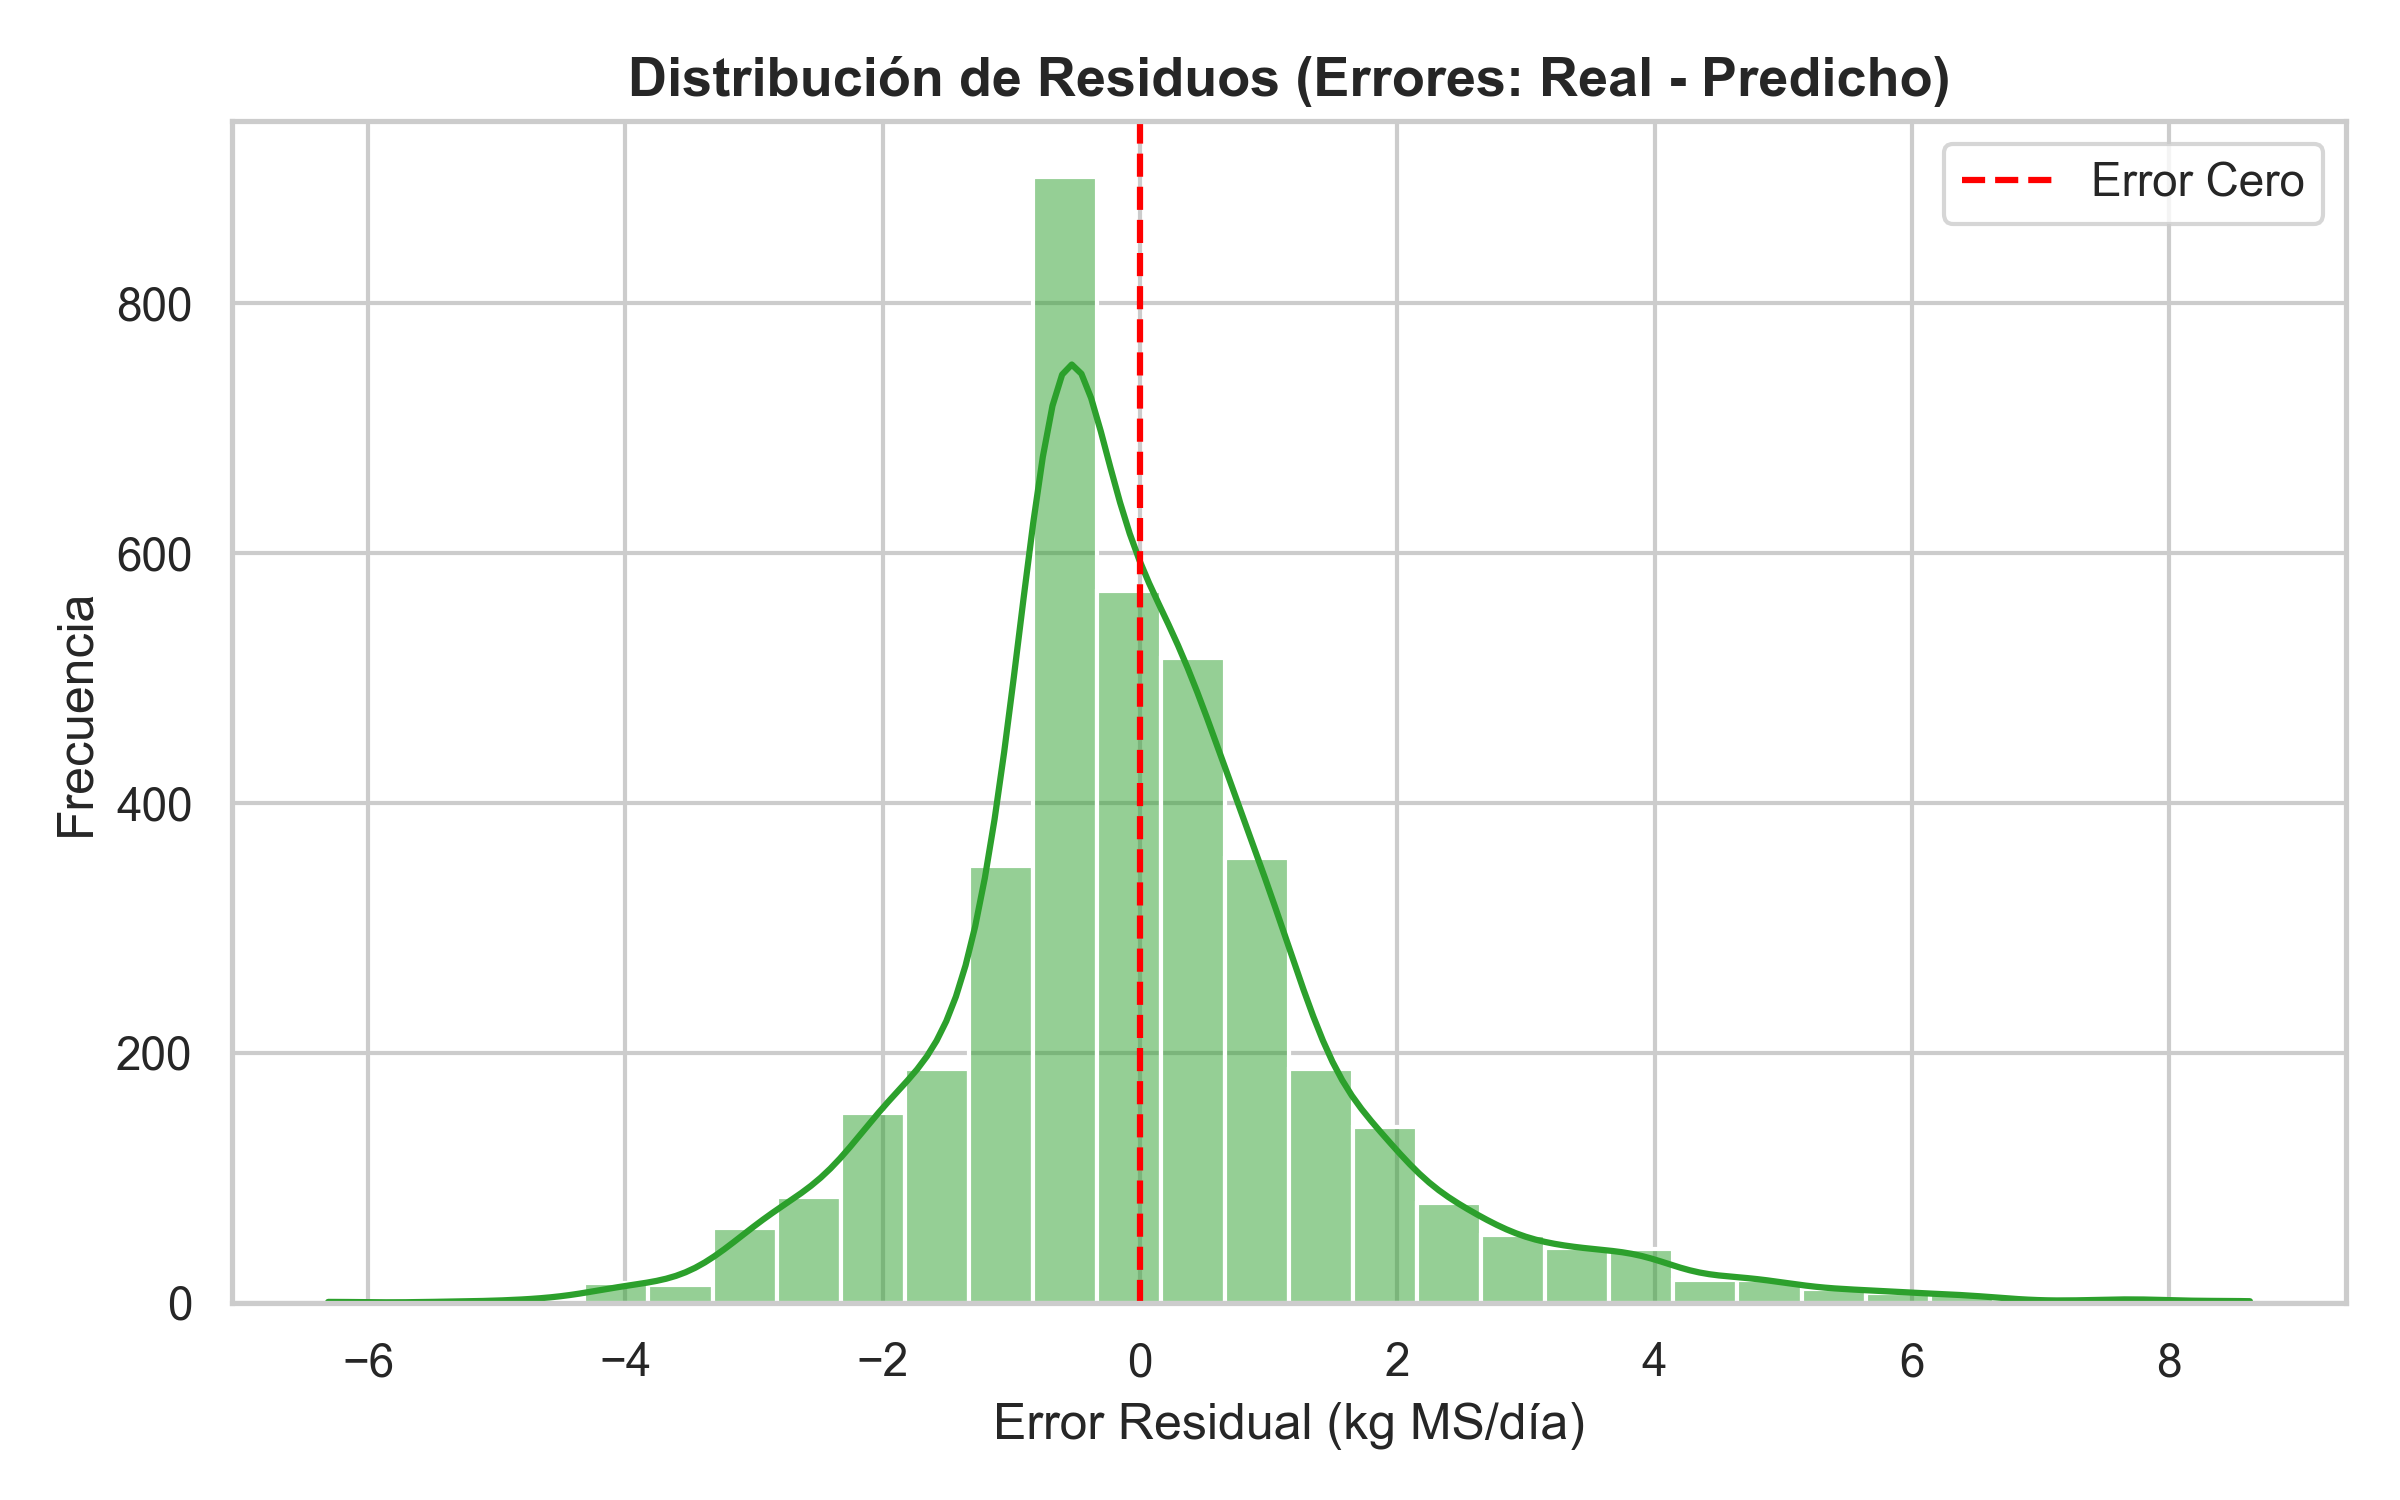
\includegraphics[width=0.9\textwidth]{figures/3_residuals_distribution.png}
\caption{Distribución de residuos de V1. Las colas muestran que algunos registros conservan errores elevados.}
\end{figure}

\subsection{Fortalezas y limitaciones de V1}

\textbf{Fortalezas:} implementación sencilla, modelo pequeño, predicción rápida, estabilidad razonable, regularización y lectura directa del pipeline.

\textbf{Limitaciones:} una única relación global debe representar categorías diferentes; la forma lineal captura con dificultad curvas, umbrales e interacciones; los coeficientes describen asociaciones y no efectos causales.

\section{Modelo V2 mejorado: ensamble por categoría}

\subsection{Motivación}

El análisis de V1 mostró que el ganador global no necesariamente era el mejor en todos los subgrupos. Las categorías tienen tamaños, distribuciones y relaciones peso-consumo distintas. V2 mejorado intenta conservar la estabilidad de Ridge y agregar flexibilidad solo donde una validación interna demuestra una mejora.

La implementación final es \codigo{CategoryBlendRegressor}. Primero calcula la predicción de Ridge V1. Luego identifica la categoría de cada fila y mezcla esa predicción con la de un especialista seleccionado para el grupo:
\begin{equation}
\hat y=(1-w)\hat y_{\text{Ridge}}+w\hat y_{\text{especialista}},\qquad 0\leq w\leq1.
\end{equation}
Si $w=0$, se conserva V1; si $w=1$, se utiliza solamente el especialista. Finalmente, la predicción se recorta a cero.

\subsection{Ingeniería de características}

Los Ridge especialistas reciben variables adicionales:
\begin{itemize}
  \item peso al cuadrado y raíz cuadrada del peso;
  \item interacción peso por condición corporal;
  \item indicadores derivados de los códigos fisiológicos;
  \item interacciones peso por lactancia y peso por preñez;
  \item interacción entre peso y cada categoría.
\end{itemize}

Peso cuadrático y raíz permiten representar curvatura. Las interacciones categoría-peso permiten pendientes diferentes. Las señales fisiológicas no se interpretan como efectos causales: son transformaciones predictivas basadas en las codificaciones utilizadas por el proyecto.

\subsection{Especialistas candidatos}

\begin{table}[H]
\centering
\caption{Familias evaluadas dentro de V2 mejorado.}
\begin{tabularx}{\textwidth}{p{4cm}X}
\toprule
\textbf{Familia} & \textbf{Configuración}\\
\midrule
Ridge V1 & Modelo base con $\alpha=10$ y entradas originales.\\
Ridge con ingeniería & Valores de $\alpha$: 0,3; 3; 10 y 100, con características fisiológicas, curvas e interacciones.\\
CatBoost RMSE & 350 iteraciones, profundidad 6, tasa 0,045, regularización L2 5 y pérdida RMSE.\\
CatBoost MAE & Misma estructura, optimizada con pérdida MAE.\\
\bottomrule
\end{tabularx}
\end{table}

La pérdida RMSE enfatiza errores grandes. La pérdida MAE se concentra en reducir el error absoluto típico. Los Ridge con distintos valores de $\alpha$ permiten ajustar el equilibrio entre flexibilidad y regularización.

\subsection{Selección del especialista y peso}

Para cada categoría se prueban pesos de mezcla desde 0 hasta 1 en incrementos de 0,05. La selección no minimiza únicamente MAE: combina las razones de MAE y RMSE frente a Ridge y agrega una penalización por la peor razón. Esto evita aceptar una reducción pequeña del error típico a costa de aumentar demasiado los errores grandes.

El enrutamiento final ajustado sobre todo el conjunto de desarrollo es:
\begin{table}[H]
\centering
\caption{Enrutamiento del artefacto final V2 mejorado.}
\begin{tabularx}{\textwidth}{p{3.2cm}X}
\toprule
\textbf{Categoría} & \textbf{Combinación seleccionada}\\
\midrule
Vaca & 55\% Ridge V1 y 45\% CatBoost con pérdida MAE.\\
Vaquilla & 75\% Ridge V1 y 25\% CatBoost con pérdida MAE.\\
Novillo & 100\% CatBoost con pérdida RMSE.\\
Toro & 100\% Ridge con ingeniería y $\alpha=100$.\\
Ternero/Ternera & 100\% Ridge con ingeniería y $\alpha=0,3$.\\
\bottomrule
\end{tabularx}
\end{table}

\subsection{Entrenamiento y validación anidada}

La evaluación utiliza cinco folds externos y tres internos. En cada fold externo:
\begin{enumerate}
  \item Se reserva un conjunto externo de prueba con hogares no vistos.
  \item Sobre el bloque restante se generan predicciones internas de todos los candidatos.
  \item Se seleccionan especialista y peso para cada categoría sin observar el fold externo.
  \item Se reentrenan los modelos seleccionados con todo el bloque externo de entrenamiento.
  \item Se predice el fold externo reservado.
\end{enumerate}

Esta estructura separa selección y evaluación. Por eso las métricas anidadas son la referencia principal para estimar generalización. Después se determina un enrutamiento final con todas las predicciones de desarrollo, se ajustan sus modelos sobre las 3.833 filas y se guarda \codigo{models/dmi_model_v2_mejorado.joblib}.

\subsection{Resultados anidados globales}

\begin{table}[H]
\centering
\caption{Resultados conservadores de V2 mejorado.}
\begin{tabular}{lr}
\toprule
\textbf{Métrica} & \textbf{Valor}\\
\midrule
MAE & 1,0791\\
RMSE & 1,5332\\
$R^2$ & 0,6830\\
Sesgo real menos predicción & 0,0796\\
Macro-MAE & 0,9050\\
Peor MAE de categoría & 1,5625\\
\bottomrule
\end{tabular}
\end{table}

El sesgo positivo de 0,0796 kg MS/día indica una subestimación promedio pequeña. El macro-MAE es el promedio simple de los cinco MAE por categoría, dando el mismo peso a cada grupo independientemente de su cantidad de filas.

\subsection{Resultados anidados por categoría}

\begin{table}[H]
\centering
\caption{V2 mejorado por categoría mediante validación anidada.}
\begin{tabular}{lrrrr}
\toprule
\textbf{Categoría} & \textbf{MAE} & \textbf{RMSE} & \textbf{$R^2$} & \textbf{Sesgo}\\
\midrule
Vaca & 1,5625 & 2,0585 & 0,4123 & 0,1544\\
Vaquilla & 0,7595 & 0,9503 & 0,5992 & 0,0062\\
Novillo & 0,6624 & 0,7974 & 0,4205 & 0,0378\\
Toro & 1,0190 & 1,4208 & 0,4651 & 0,1042\\
Ternero/Ternera & 0,5216 & 0,6529 & 0,6415 & -0,0014\\
\bottomrule
\end{tabular}
\end{table}

Ternero/Ternera presenta el beneficio más claro. Vaquilla no mejora en la evaluación anidada. Toro conserva un MAE prácticamente igual a V1, pero empeora RMSE y $R^2$, señal de algunos errores grandes o menor estabilidad.

\subsection{Lectura de métricas: qué significan y qué tan buenas son}

La lectura principal utiliza la validación anidada, porque selecciona especialistas sin observar el fold externo de prueba. Los porcentajes de error vuelven a calcularse sobre el DMI medio de 4,8285 kg MS/día.

\begin{table}[H]
\centering
\caption{Lectura práctica de las métricas globales de V2 mejorado.}
\begin{tabularx}{\textwidth}{p{2.5cm}p{2.8cm}X}
\toprule
\textbf{Métrica} & \textbf{Lectura porcentual} & \textbf{Interpretación}\\
\midrule
MAE 1,0791 & 22,35\% del DMI medio & El error absoluto típico es aproximadamente 1,08 kg MS/día. Es el menor MAE global de los dos modelos finales.\\
RMSE 1,5332 & 31,75\% del DMI medio & Los errores grandes siguen siendo relevantes. La reducción frente a V1 es muy pequeña, por lo que este aspecto permanece prácticamente igual.\\
$R^2=0,6830$ & 68,30\% de la variabilidad representada & El modelo captura algo más de dos tercios de la variabilidad del DMI. No equivale a 68,30\% de predicciones correctas.\\
Sesgo 0,0796 & 1,65\% del DMI medio & En promedio, el valor real supera a la predicción en 0,0796 kg MS/día; existe una subestimación global pequeña.\\
\bottomrule
\end{tabularx}
\end{table}

Frente a V1, V2 mejorado reduce el MAE \textbf{2,07\%}, reduce el RMSE \textbf{0,14\%} y aumenta el $R^2$ aproximadamente \textbf{0,13\% en términos relativos}. La mejora de $R^2$ es de 0,0009 puntos, por lo que no debe describirse como un salto importante.

\begin{table}[H]
\centering
\caption{Cambio porcentual del MAE de V2 mejorado respecto de V1.}
\begin{tabular}{lrl}
\toprule
\textbf{Categoría} & \textbf{Cambio MAE} & \textbf{Lectura}\\
\midrule
Vaca & -1,46\% & Mejora pequeña.\\
Vaquilla & +0,73\% & Empeoramiento pequeño.\\
Novillo & -0,23\% & Resultado prácticamente igual.\\
Toro & -0,14\% & MAE casi igual; RMSE y $R^2$ empeoran.\\
Ternero/Ternera & -10,78\% & Mejora clara y principal aporte del ensamble.\\
\bottomrule
\end{tabular}
\end{table}

\subsubsection{Lectura por categoría}

Los porcentajes siguientes utilizan el consumo medio propio de cada categoría y las métricas de validación anidada. Esta es la comparación más prudente, porque cada especialista fue seleccionado sin observar el fold externo evaluado.

\begin{table}[H]
\centering
\caption{Lectura relativa de V2 mejorado por categoría.}
\resizebox{\textwidth}{!}{%
\begin{tabular}{lrrrrl}
\toprule
\textbf{Categoría} & \textbf{DMI medio} & \textbf{MAE relativo} & \textbf{RMSE relativo} & \textbf{$R^2$} & \textbf{Valoración}\\
\midrule
Vaca & 6,6177 & 23,61\% & 31,11\% & 41,23\% & Moderada; mejora pequeña frente a V1.\\
Vaquilla & 3,9438 & 19,26\% & 24,10\% & 59,92\% & Buena, pero ligeramente inferior a V1.\\
Novillo & 3,6185 & 18,31\% & 22,04\% & 42,05\% & Buen error relativo; mejora mínima.\\
Toro & 5,0970 & 19,99\% & 27,88\% & 46,51\% & Mixta; MAE estable y errores grandes peores.\\
Ternero/Ternera & 2,2183 & 23,51\% & 29,43\% & 64,15\% & Buena y claramente mejor que V1.\\
\bottomrule
\end{tabular}}
\end{table}

\begin{itemize}
  \item \textbf{Vaca:} el MAE equivale al 23,61\% del consumo medio y el $R^2$ es 41,23\%. La mejora sobre V1 existe, pero es pequeña; el grupo continúa siendo difícil.
  \item \textbf{Vaquilla:} mantiene una lectura buena, con MAE relativo de 19,26\% y $R^2$ de 59,92\%, pero las tres métricas son ligeramente peores que las de V1. El especialista no aporta una ventaja confirmada.
  \item \textbf{Novillo:} logra el menor MAE relativo, 18,31\%, y un $R^2$ de 42,05\%. La mejora frente a V1 es mínima, por lo que ambos modelos son prácticamente equivalentes en este grupo.
  \item \textbf{Toro:} el MAE relativo queda casi igual en 19,99\%, pero el RMSE relativo sube a 27,88\% y el $R^2$ baja a 46,51\%. La lectura es mixta: el error típico no empeora, pero algunos errores grandes sí.
  \item \textbf{Ternero/Ternera:} el MAE relativo baja de 26,35\% a 23,51\%, el RMSE relativo baja a 29,43\% y el $R^2$ sube a 64,15\%. Es la mejora más clara y la categoría donde V2 mejorado demuestra mayor utilidad.
\end{itemize}

\textbf{¿Qué tan bueno es V2 mejorado?} Es el \textbf{mejor modelo disponible por resultados} y su rendimiento global puede calificarse como bueno dentro de esta evaluación interna. Sin embargo, es solo \textbf{ligeramente mejor que V1} en el agregado. La evidencia es convincente para Ternero/Ternera, moderada para Vaca y débil o desfavorable para Vaquilla, Novillo y Toro. Por eso no corresponde llamarlo excelente ni afirmar que mejora todos los tipos de animal.

La calidad continúa limitada por un error típico equivalente al 22,35\% del consumo medio, por variables relevantes que no están disponibles y por la ausencia de validación externa. Su ventaja debe entenderse como una optimización moderada del mejor modelo anterior, no como una solución definitiva.

\subsection{Estabilidad por fold externo}

\begin{table}[H]
\centering
\caption{Resultados de V2 mejorado en los cinco folds externos.}
\begin{tabular}{crrrr}
\toprule
\textbf{Fold} & \textbf{MAE} & \textbf{RMSE} & \textbf{$R^2$} & \textbf{Sesgo}\\
\midrule
1 & 1,0892 & 1,5178 & 0,6700 & -0,0313\\
2 & 1,0821 & 1,5413 & 0,7198 & 0,1222\\
3 & 1,1310 & 1,5966 & 0,6859 & 0,1319\\
4 & 1,0489 & 1,4931 & 0,6796 & 0,0542\\
5 & 1,0484 & 1,5204 & 0,6294 & 0,1202\\
\bottomrule
\end{tabular}
\end{table}

El enrutamiento elegido cambia parcialmente entre folds, especialmente en categorías con menos hogares. Esto confirma que la especialización aporta flexibilidad, pero también aumenta incertidumbre de selección.

\subsection{Resultado de desarrollo}

El artefacto final fijo obtiene MAE 1,0746, RMSE 1,5266, $R^2=0,6858$ y sesgo 0,0767 en predicciones fuera de fold de desarrollo. Estos números describen el enrutamiento finalmente seleccionado, pero participaron en la elección de esa configuración. Por esta razón se informan como resultado secundario y no sustituyen la validación anidada.

\begin{figure}[H]
\centering
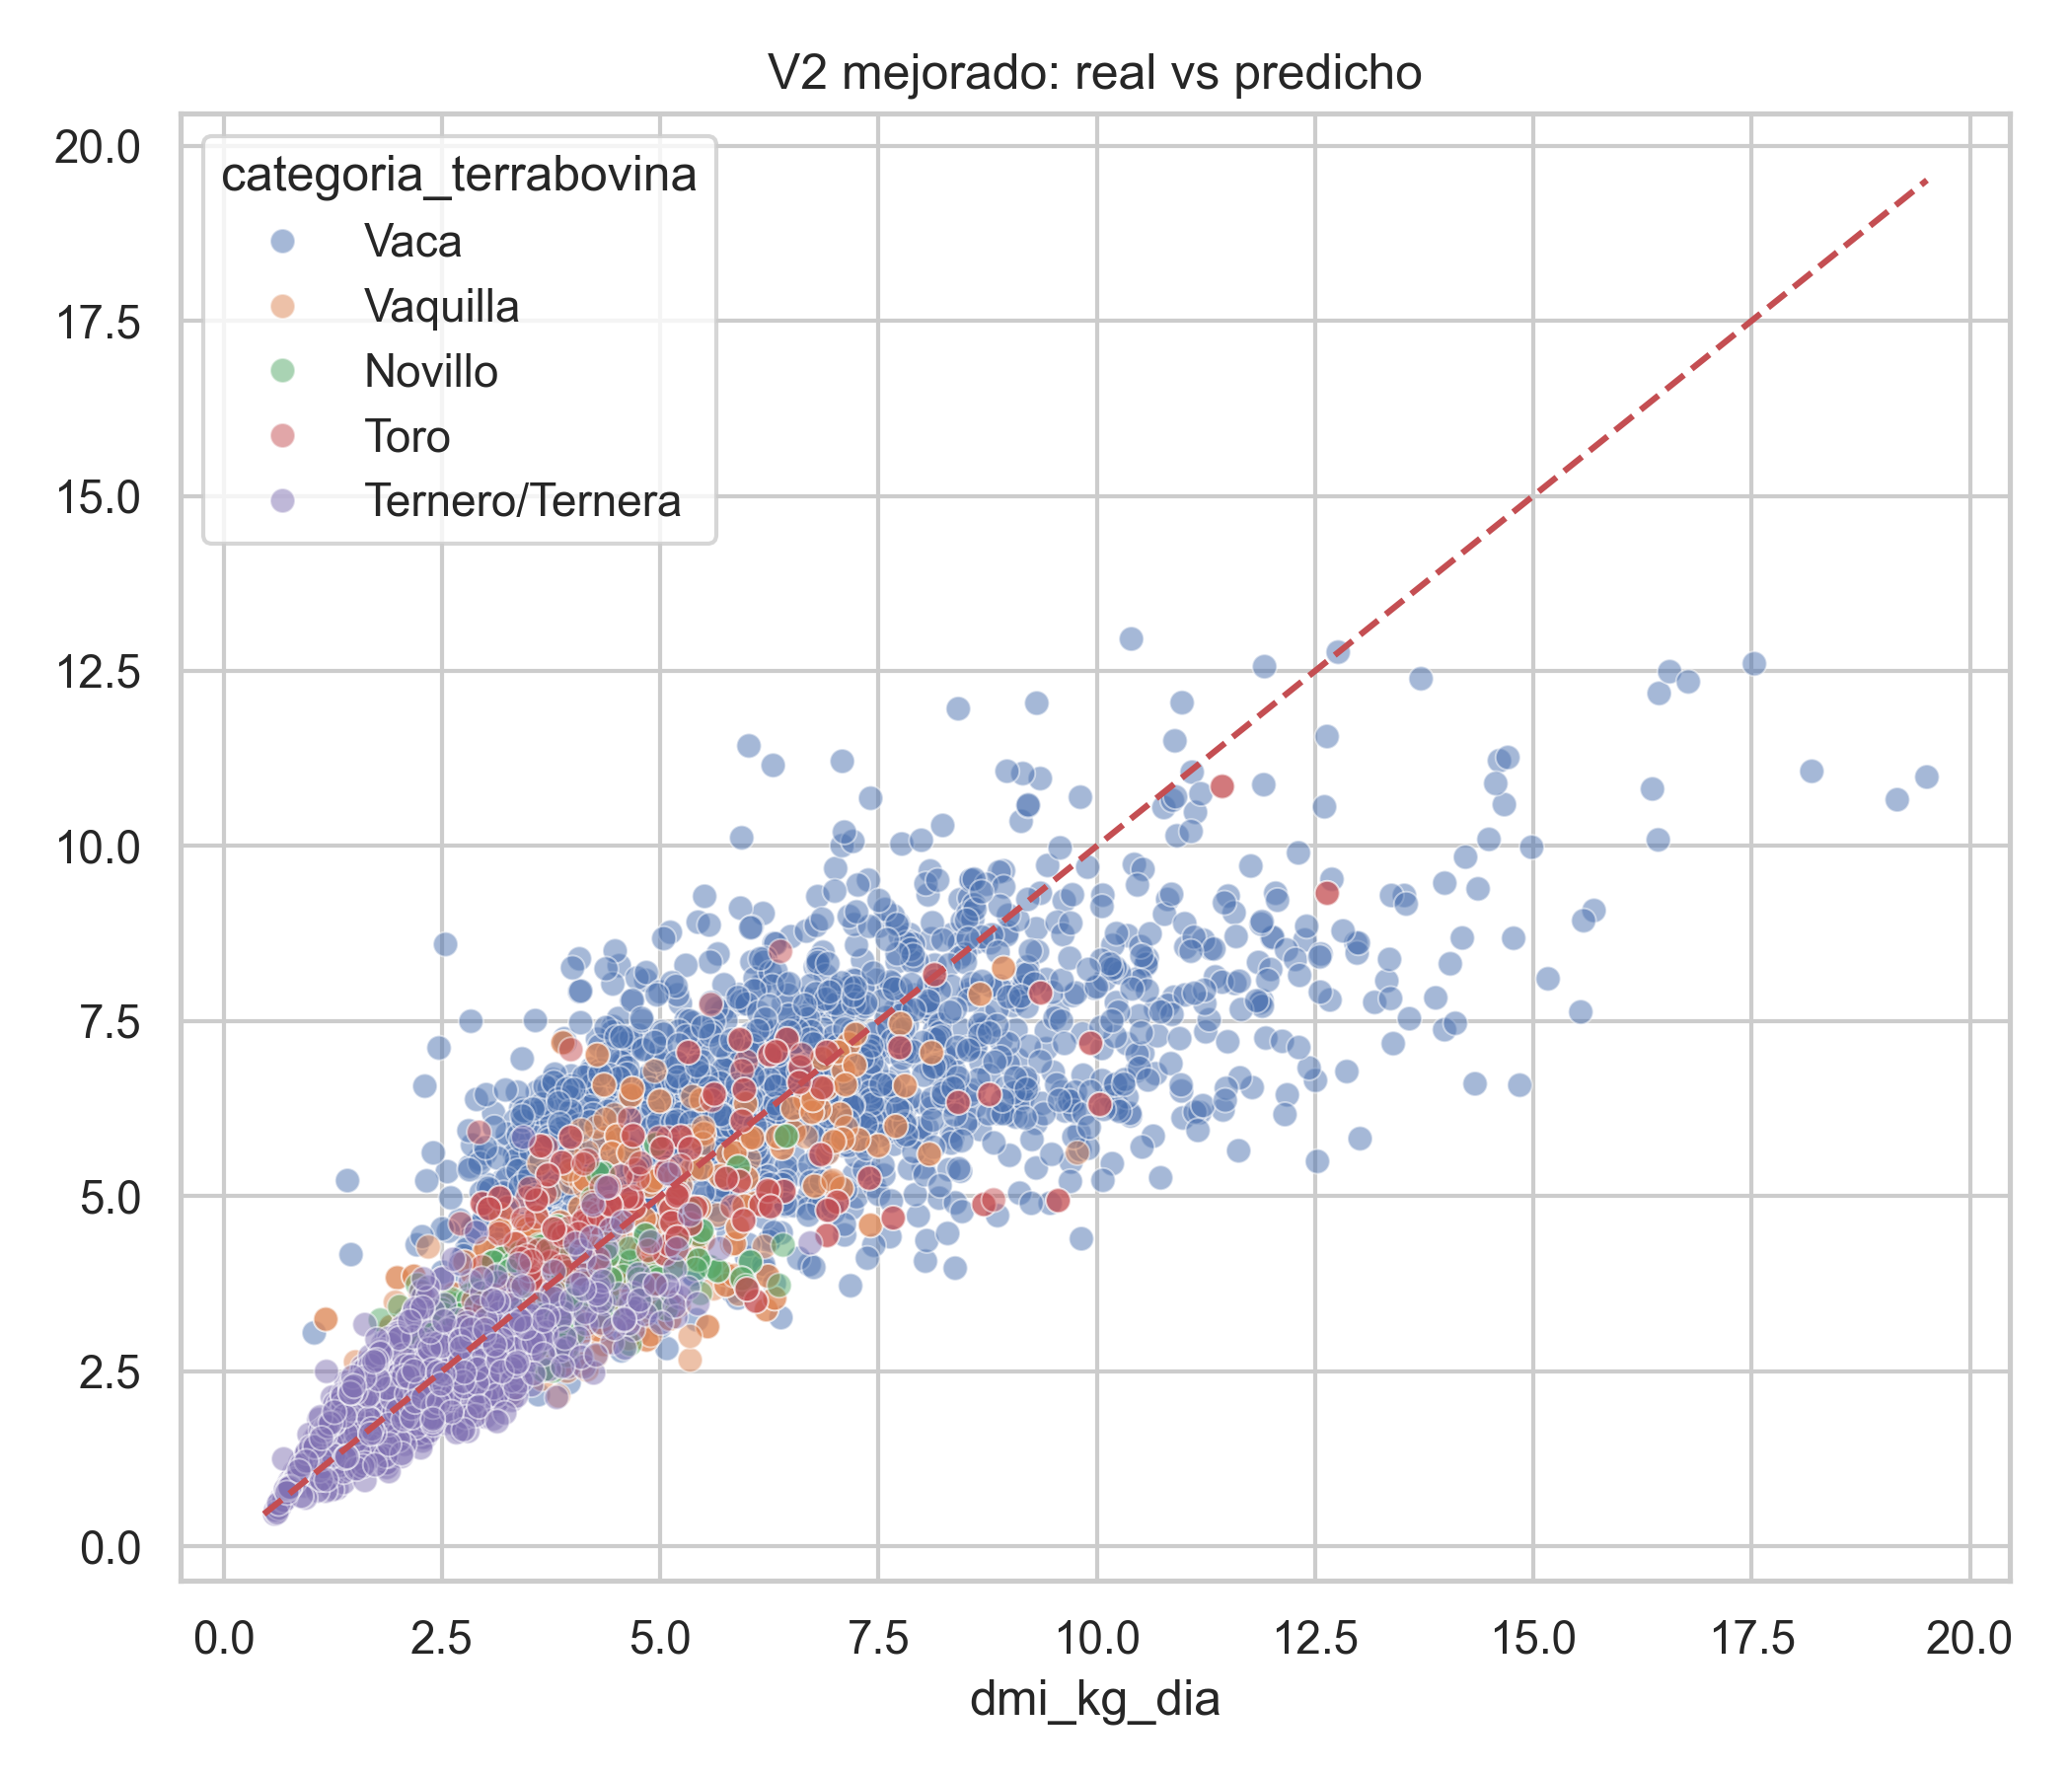
\includegraphics[width=0.84\textwidth]{figures_v2_mejorado/5_actual_vs_predicted.png}
\caption{DMI real frente a predicciones fuera de fold del enrutamiento final de V2 mejorado.}
\end{figure}

\subsection{Fortalezas y limitaciones de V2 mejorado}

\textbf{Fortalezas:} adapta el modelo a categorías heterogéneas, conserva Ridge donde conviene, permite relaciones curvas e interacciones, controla la selección mediante validación anidada y mejora el MAE global.

\textbf{Limitaciones:} mayor complejidad, más modelos almacenados, mayor costo de entrenamiento, enrutamiento sensible en grupos pequeños y mejoras no uniformes. Su reporte lo identifica como versión experimental.

\section{Comparación final}

\subsection{Comparación global principal}

\begin{table}[H]
\centering
\caption{V1 frente a V2 mejorado con evaluación anidada.}
\begin{tabular}{lrrrr}
\toprule
\textbf{Métrica} & \textbf{V1 Ridge} & \textbf{V2 mejorado} & \textbf{Cambio} & \textbf{Cambio relativo}\\
\midrule
MAE $\downarrow$ & 1,1019 & \textbf{1,0791} & -0,0228 & -2,07\%\\
RMSE $\downarrow$ & 1,5354 & \textbf{1,5332} & -0,0022 & -0,14\%\\
$R^2$ $\uparrow$ & 0,6821 & \textbf{0,6830} & +0,0009 & +0,13\%\\
\bottomrule
\end{tabular}
\end{table}

Las tres métricas globales cambian en dirección favorable, pero el margen es reducido. La evidencia más práctica es la disminución de MAE: el error absoluto promedio baja 0,0228 kg MS/día, alrededor de 22,8 gramos diarios por observación. La mejora relativa es aproximadamente 2,07\%.

\begin{figure}[H]
\centering
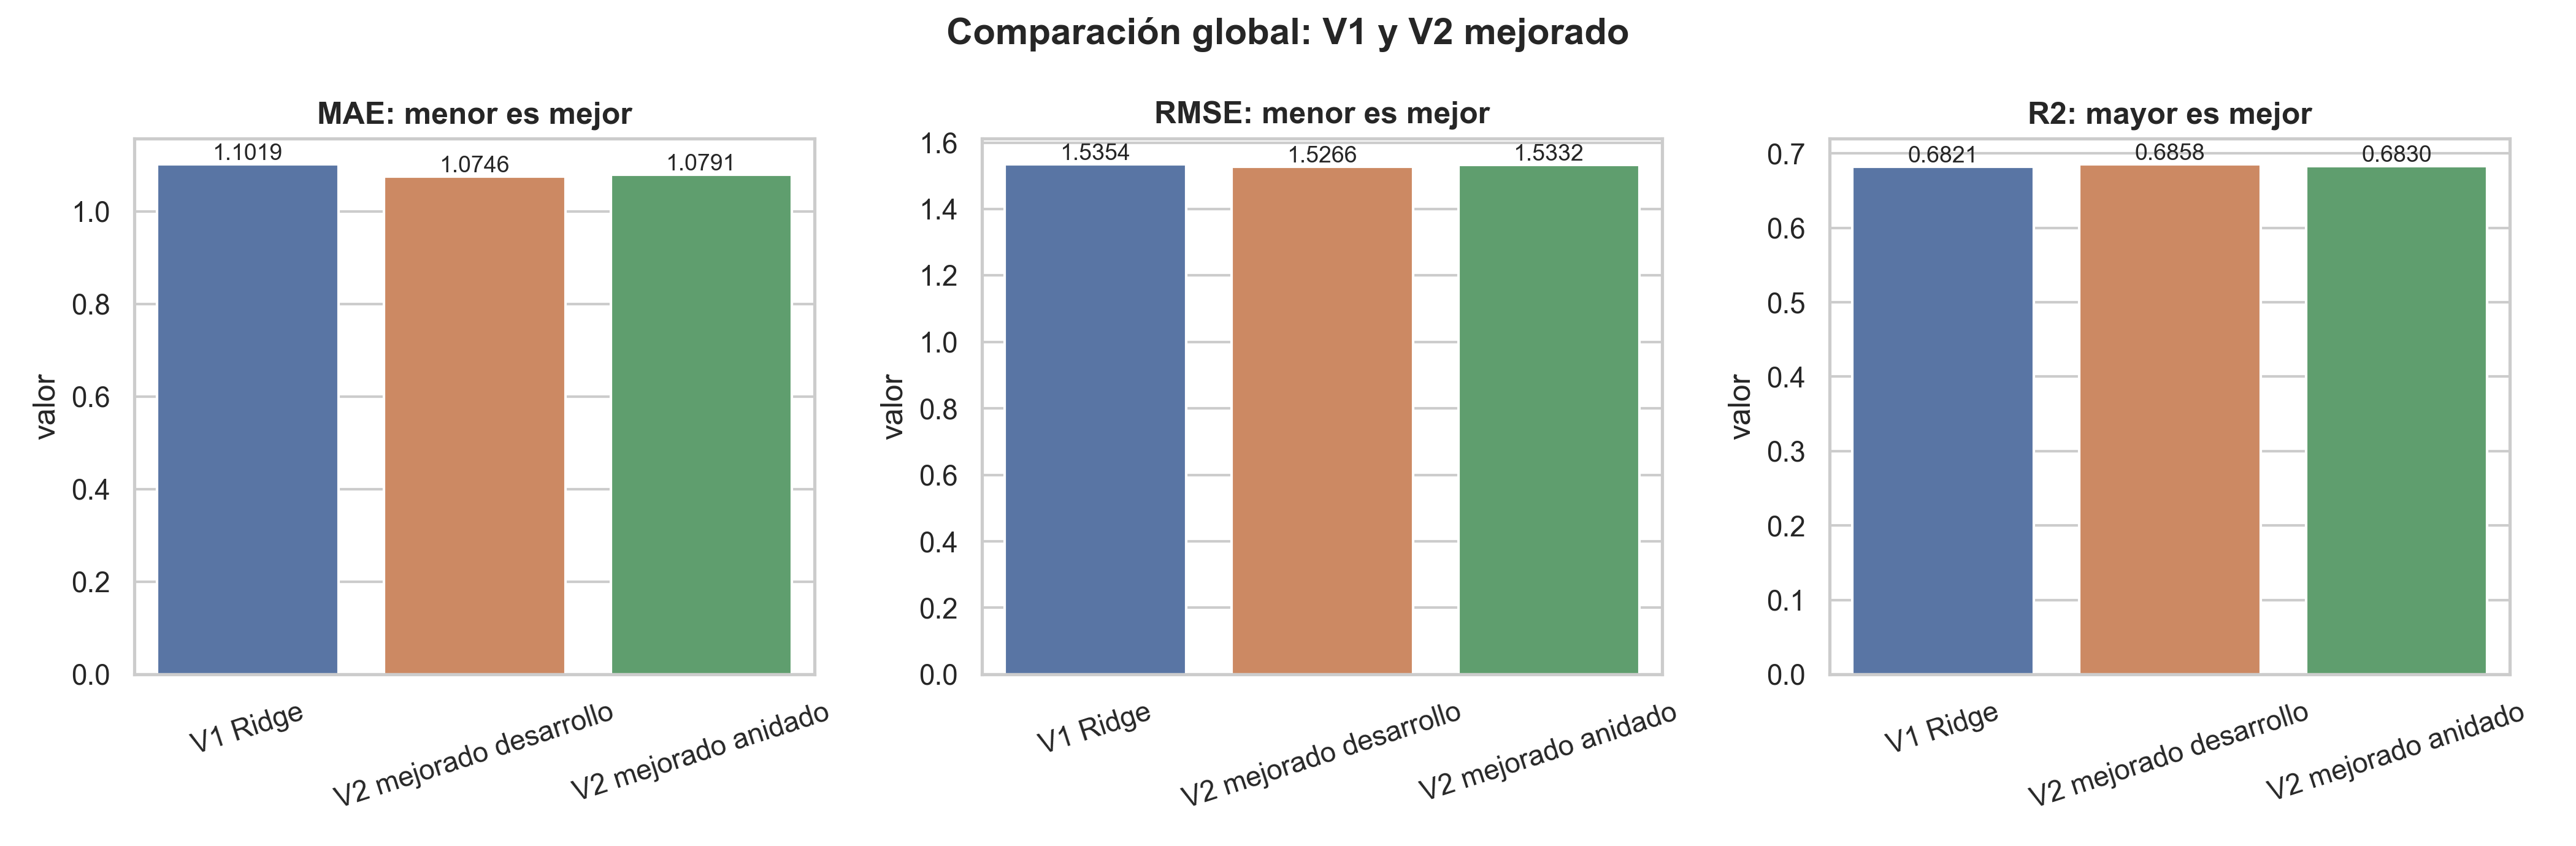
\includegraphics[width=\textwidth]{figures_metricas_detalladas/1_global_tres_evaluaciones.png}
\caption{Comparación global entre V1, el enrutamiento final de desarrollo y la evaluación anidada de V2 mejorado.}
\end{figure}

\subsection{Comparación por categoría}

\begin{table}[H]
\centering
\caption{Comparación anidada por categoría.}
\resizebox{\textwidth}{!}{%
\begin{tabular}{lrrrrrrrrr}
\toprule
& \multicolumn{3}{c}{\textbf{V1 Ridge}} & \multicolumn{3}{c}{\textbf{V2 mejorado}} & \multicolumn{3}{c}{\textbf{Cambio V2 mejorado - V1}}\\
\cmidrule(lr){2-4}\cmidrule(lr){5-7}\cmidrule(lr){8-10}
\textbf{Categoría} & MAE & RMSE & $R^2$ & MAE & RMSE & $R^2$ & MAE & RMSE & $R^2$\\
\midrule
Vaca & 1,5857 & 2,0608 & 0,4110 & 1,5625 & 2,0585 & 0,4123 & -0,0232 & -0,0023 & +0,0013\\
Vaquilla & 0,7540 & 0,9449 & 0,6037 & 0,7595 & 0,9503 & 0,5992 & +0,0055 & +0,0054 & -0,0045\\
Novillo & 0,6639 & 0,8028 & 0,4126 & 0,6624 & 0,7974 & 0,4205 & -0,0015 & -0,0054 & +0,0079\\
Toro & 1,0204 & 1,3642 & 0,5068 & 1,0190 & 1,4208 & 0,4651 & -0,0014 & +0,0566 & -0,0417\\
Ternero/Ternera & 0,5846 & 0,7018 & 0,5858 & 0,5216 & 0,6529 & 0,6415 & -0,0630 & -0,0489 & +0,0557\\
\bottomrule
\end{tabular}}
\end{table}

La tabla muestra por qué no debe resumirse la decisión como una victoria uniforme. V2 mejorado gana claramente en Ternero/Ternera, mejora de forma pequeña en Vaca y Novillo, retrocede levemente en Vaquilla y produce una lectura mixta en Toro.

\begin{figure}[H]
\centering
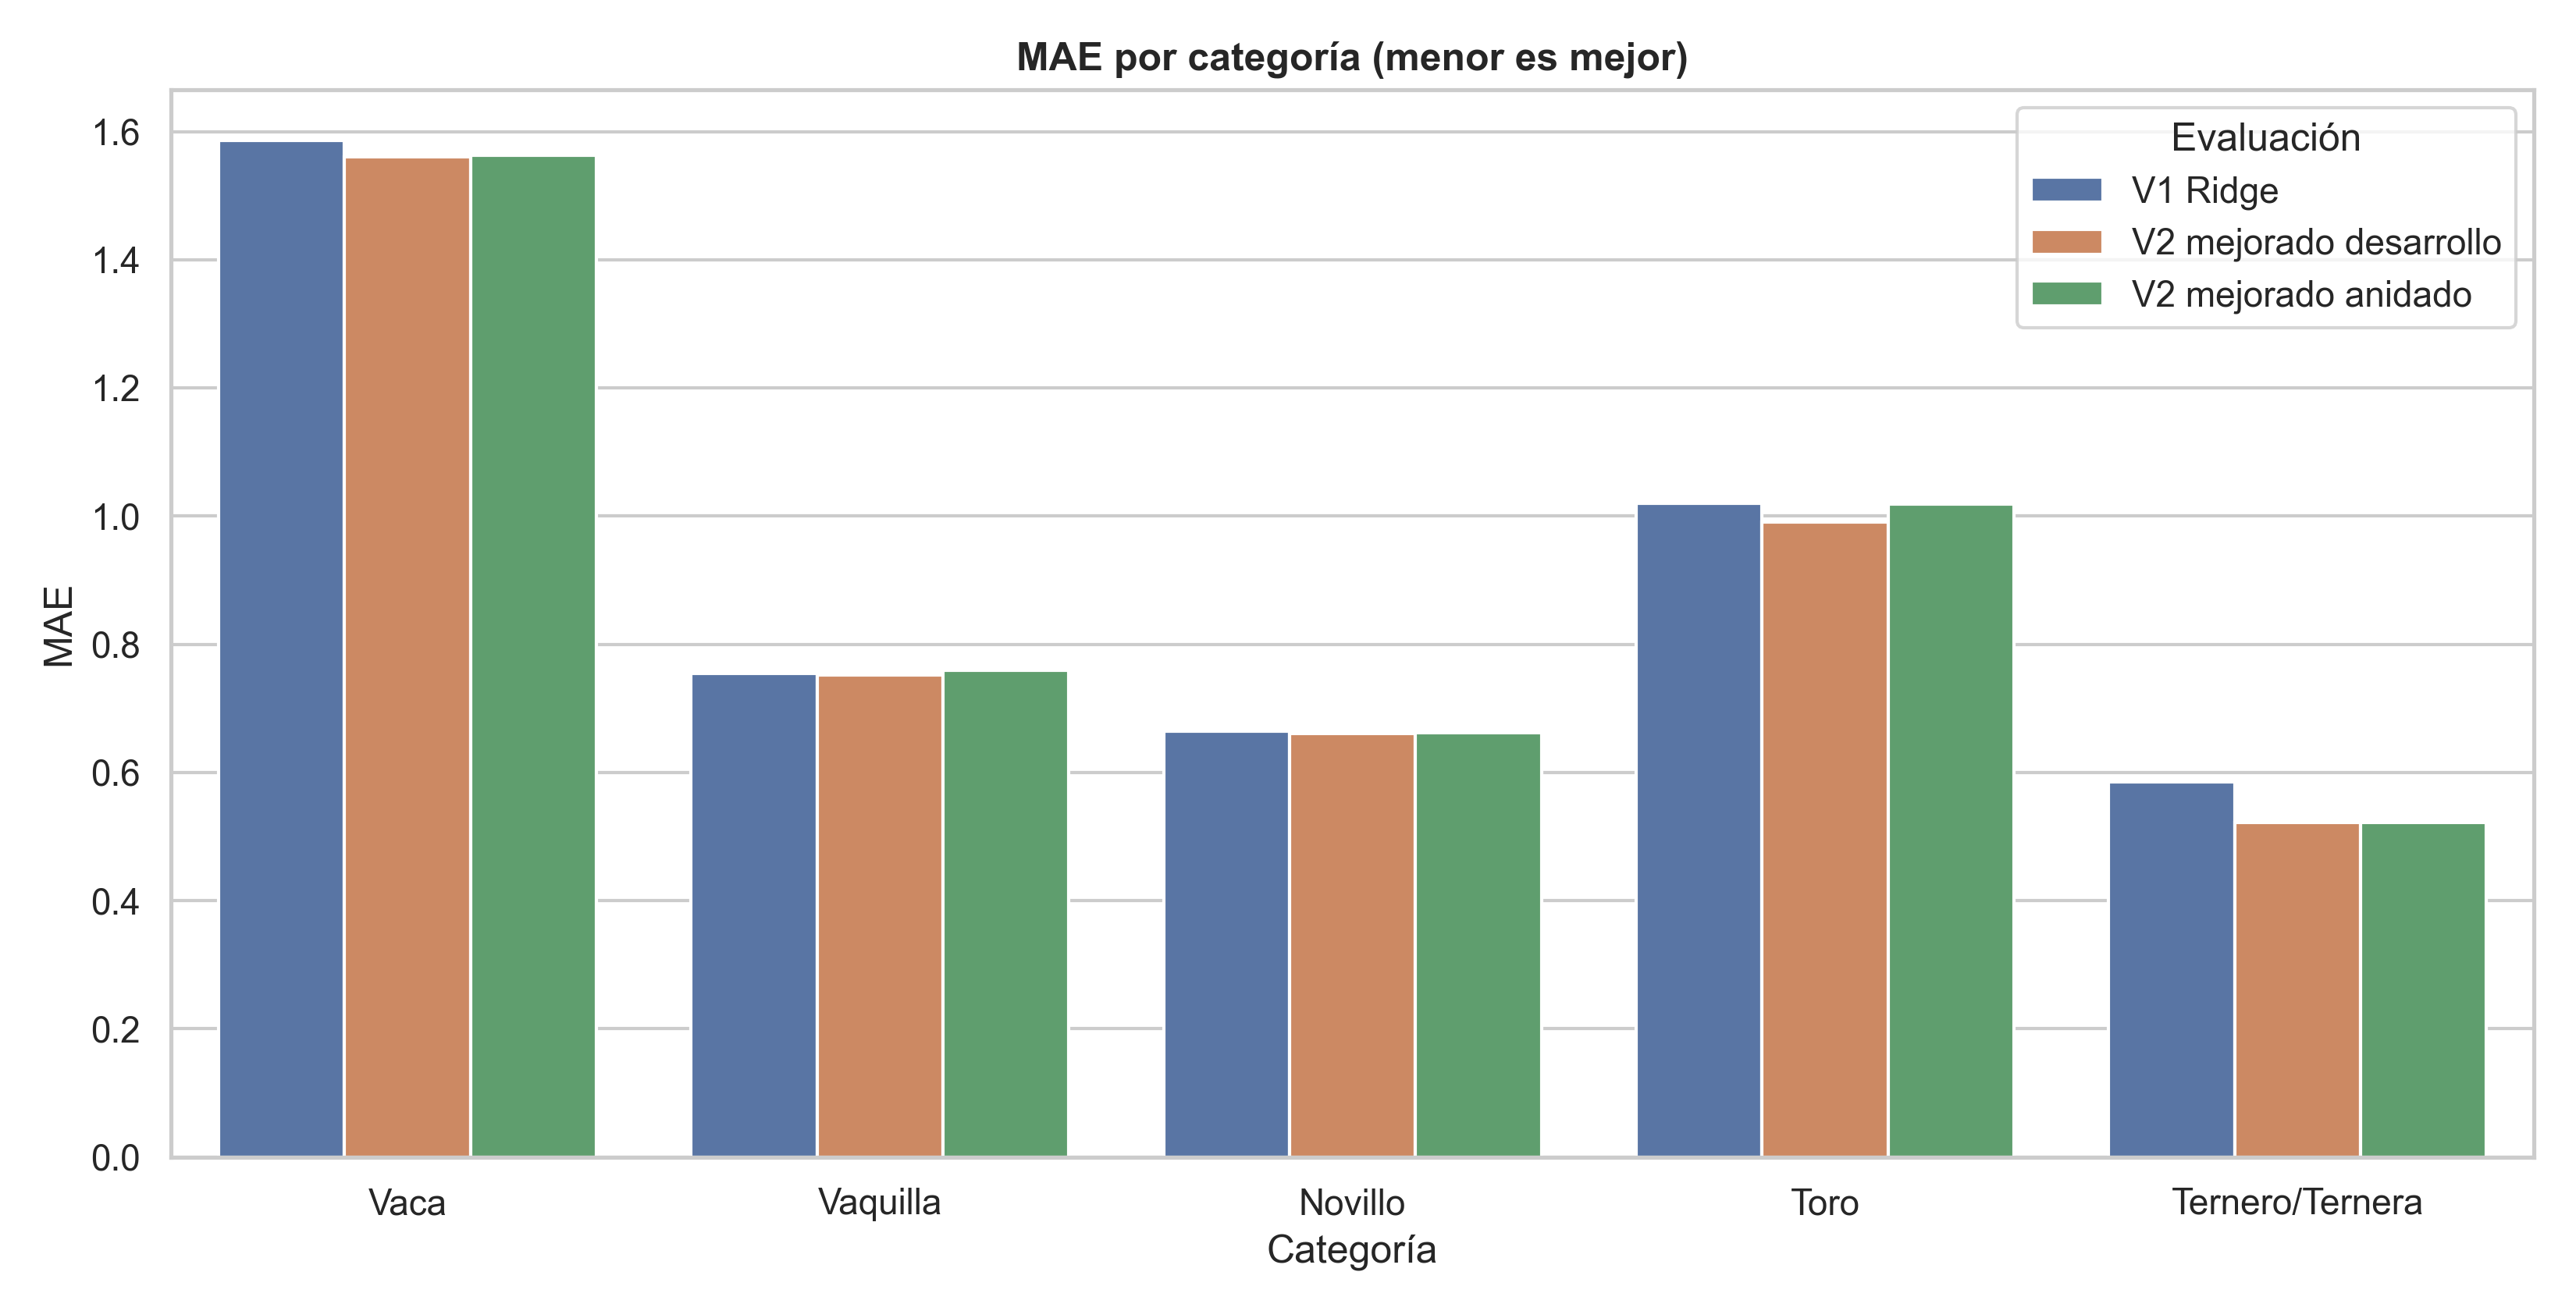
\includegraphics[width=0.95\textwidth]{figures_metricas_detalladas/2_mae_categoria.png}
\caption{MAE por categoría. Menor es mejor.}
\end{figure}

\begin{figure}[H]
\centering
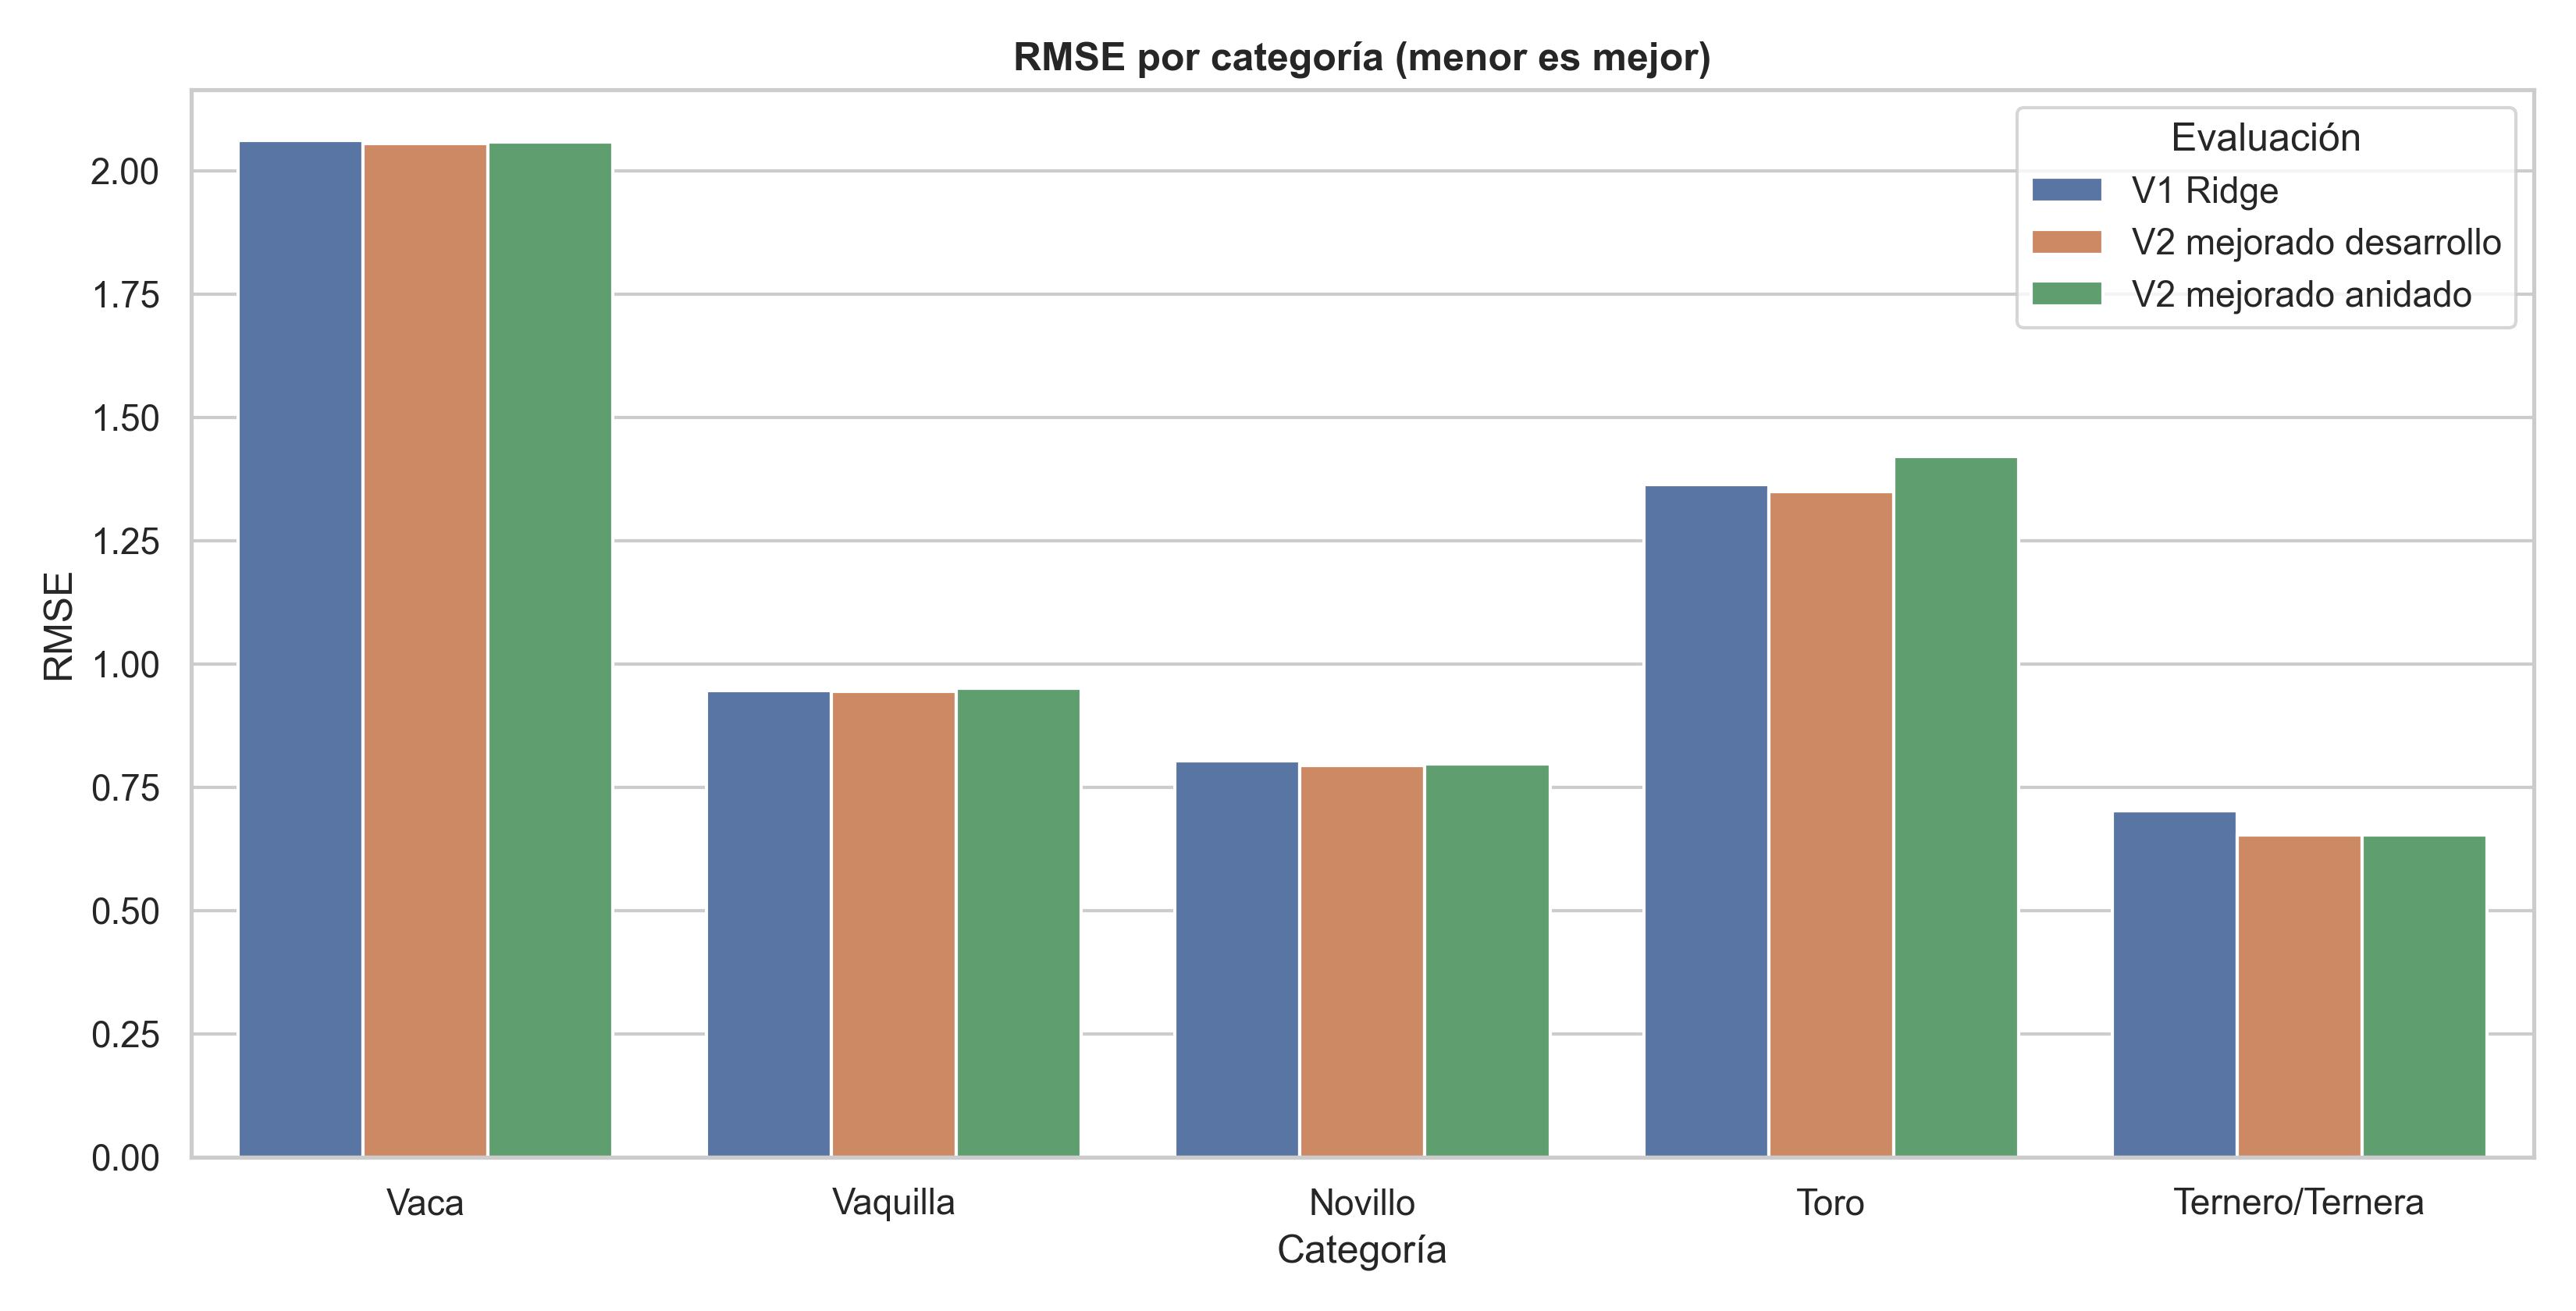
\includegraphics[width=0.95\textwidth]{figures_metricas_detalladas/3_rmse_categoria.png}
\caption{RMSE por categoría. La evaluación anidada evidencia el retroceso de Toro en errores grandes.}
\end{figure}

\begin{figure}[H]
\centering
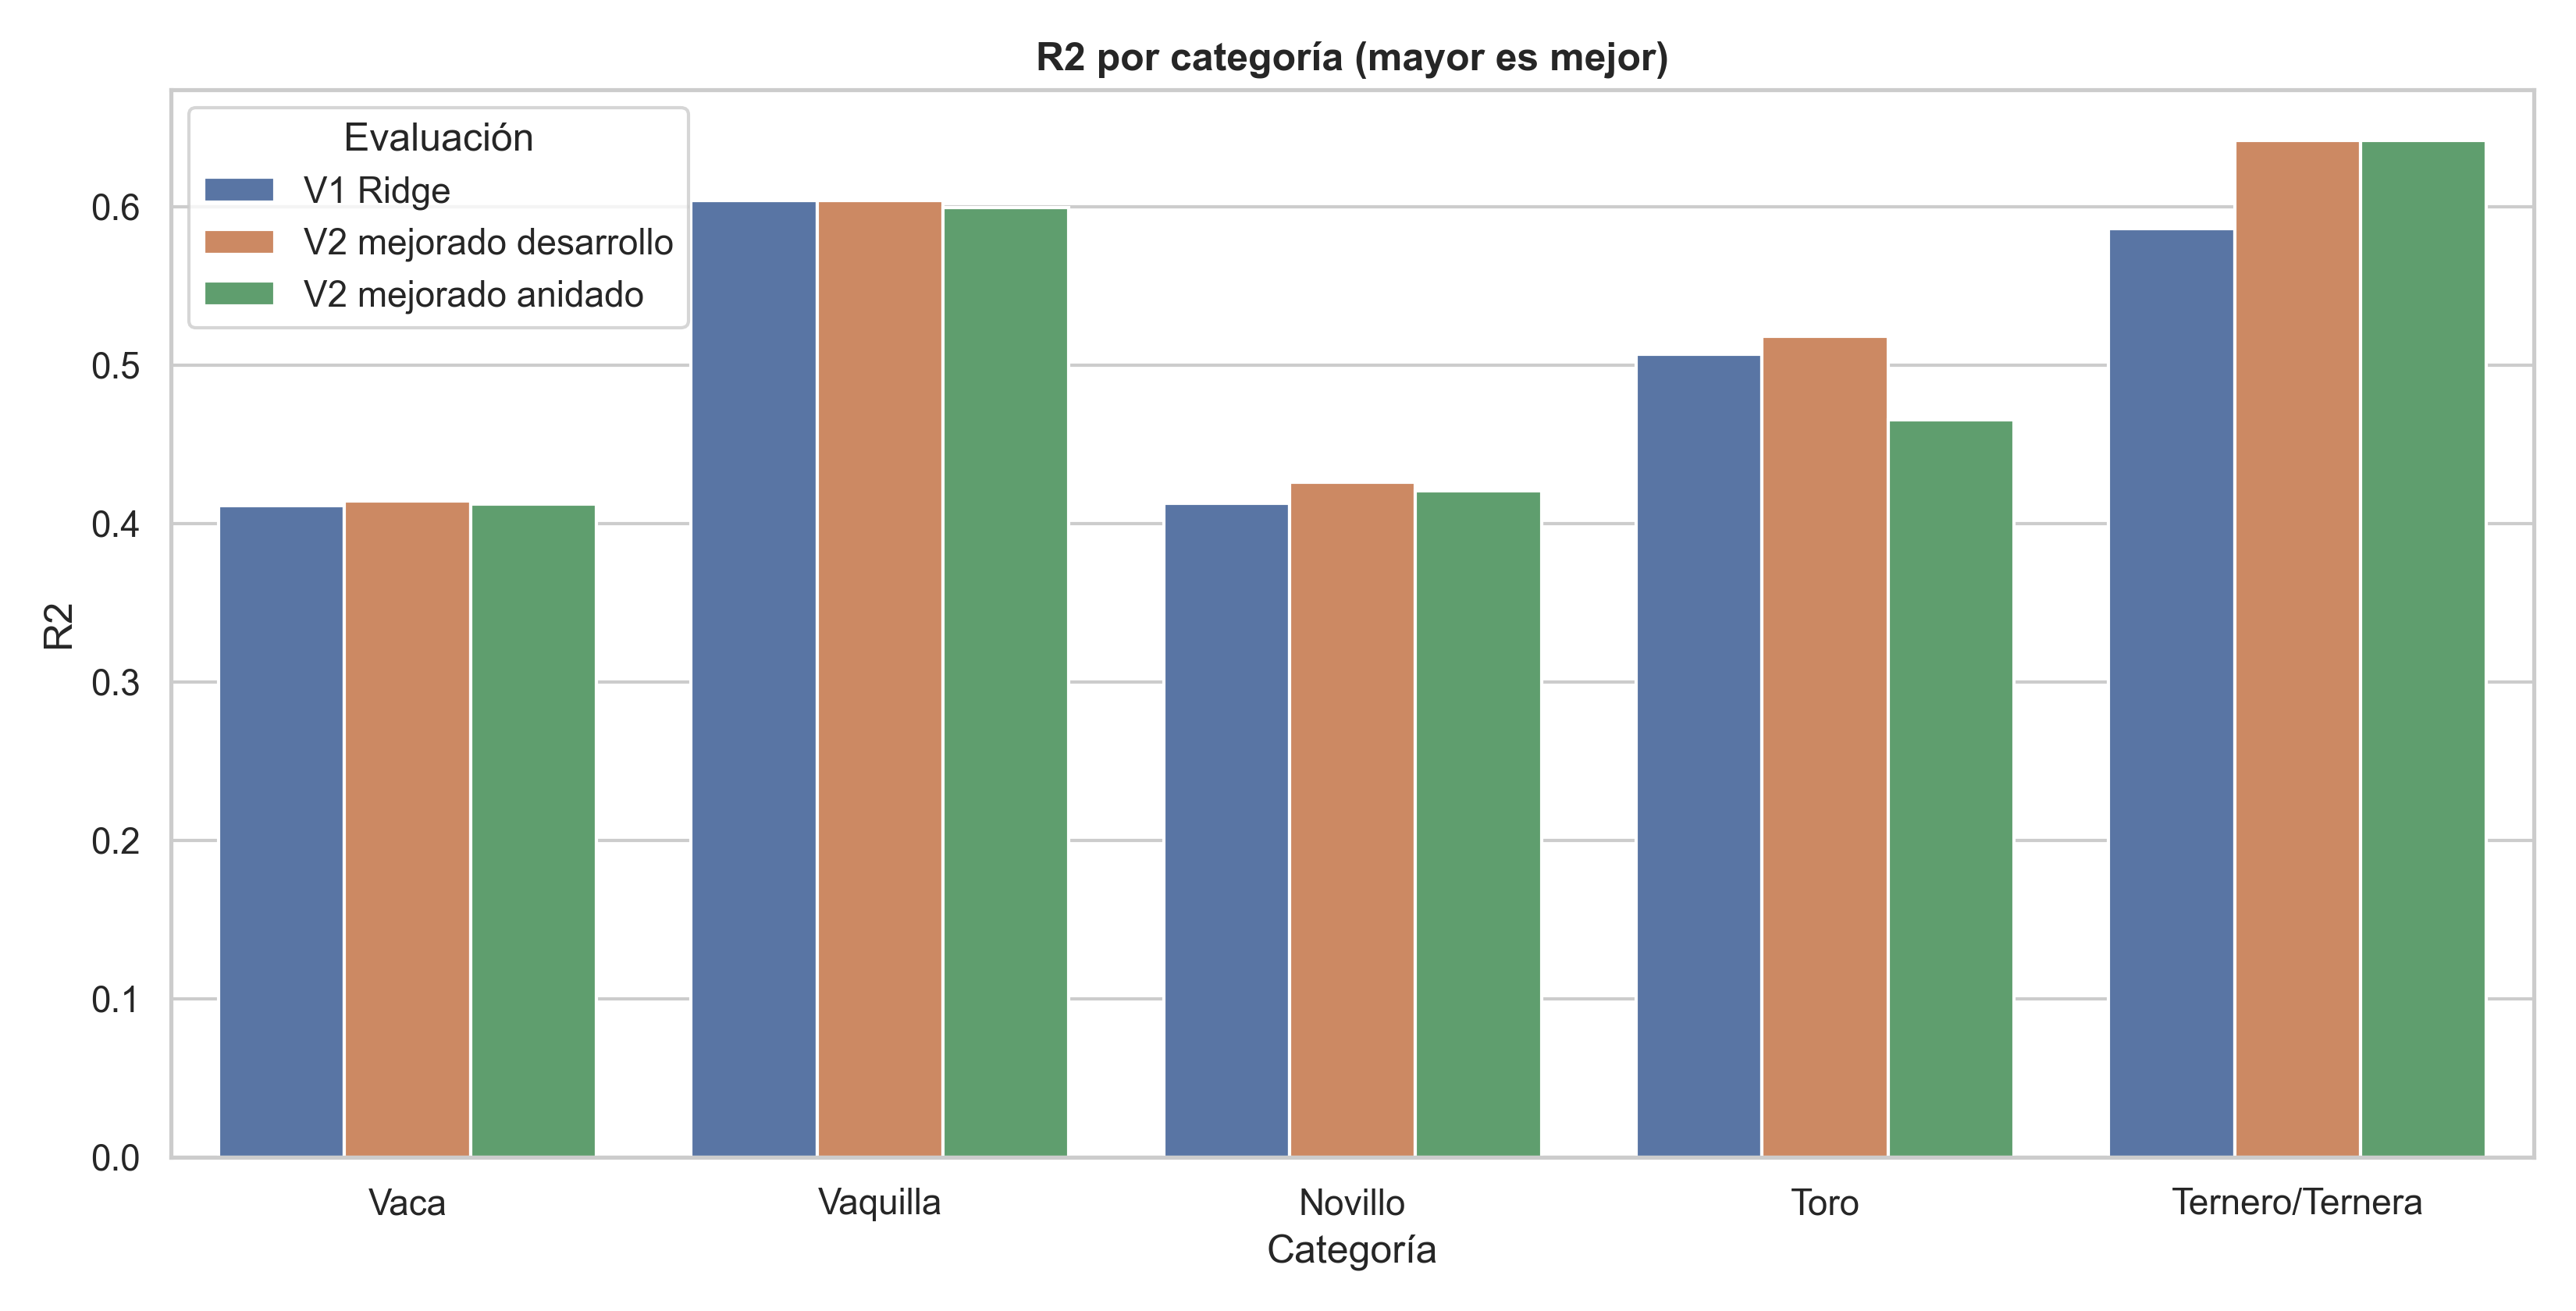
\includegraphics[width=0.95\textwidth]{figures_metricas_detalladas/4_r2_categoria.png}
\caption{$R^2$ por categoría. Mayor es mejor.}
\end{figure}

\begin{figure}[H]
\centering
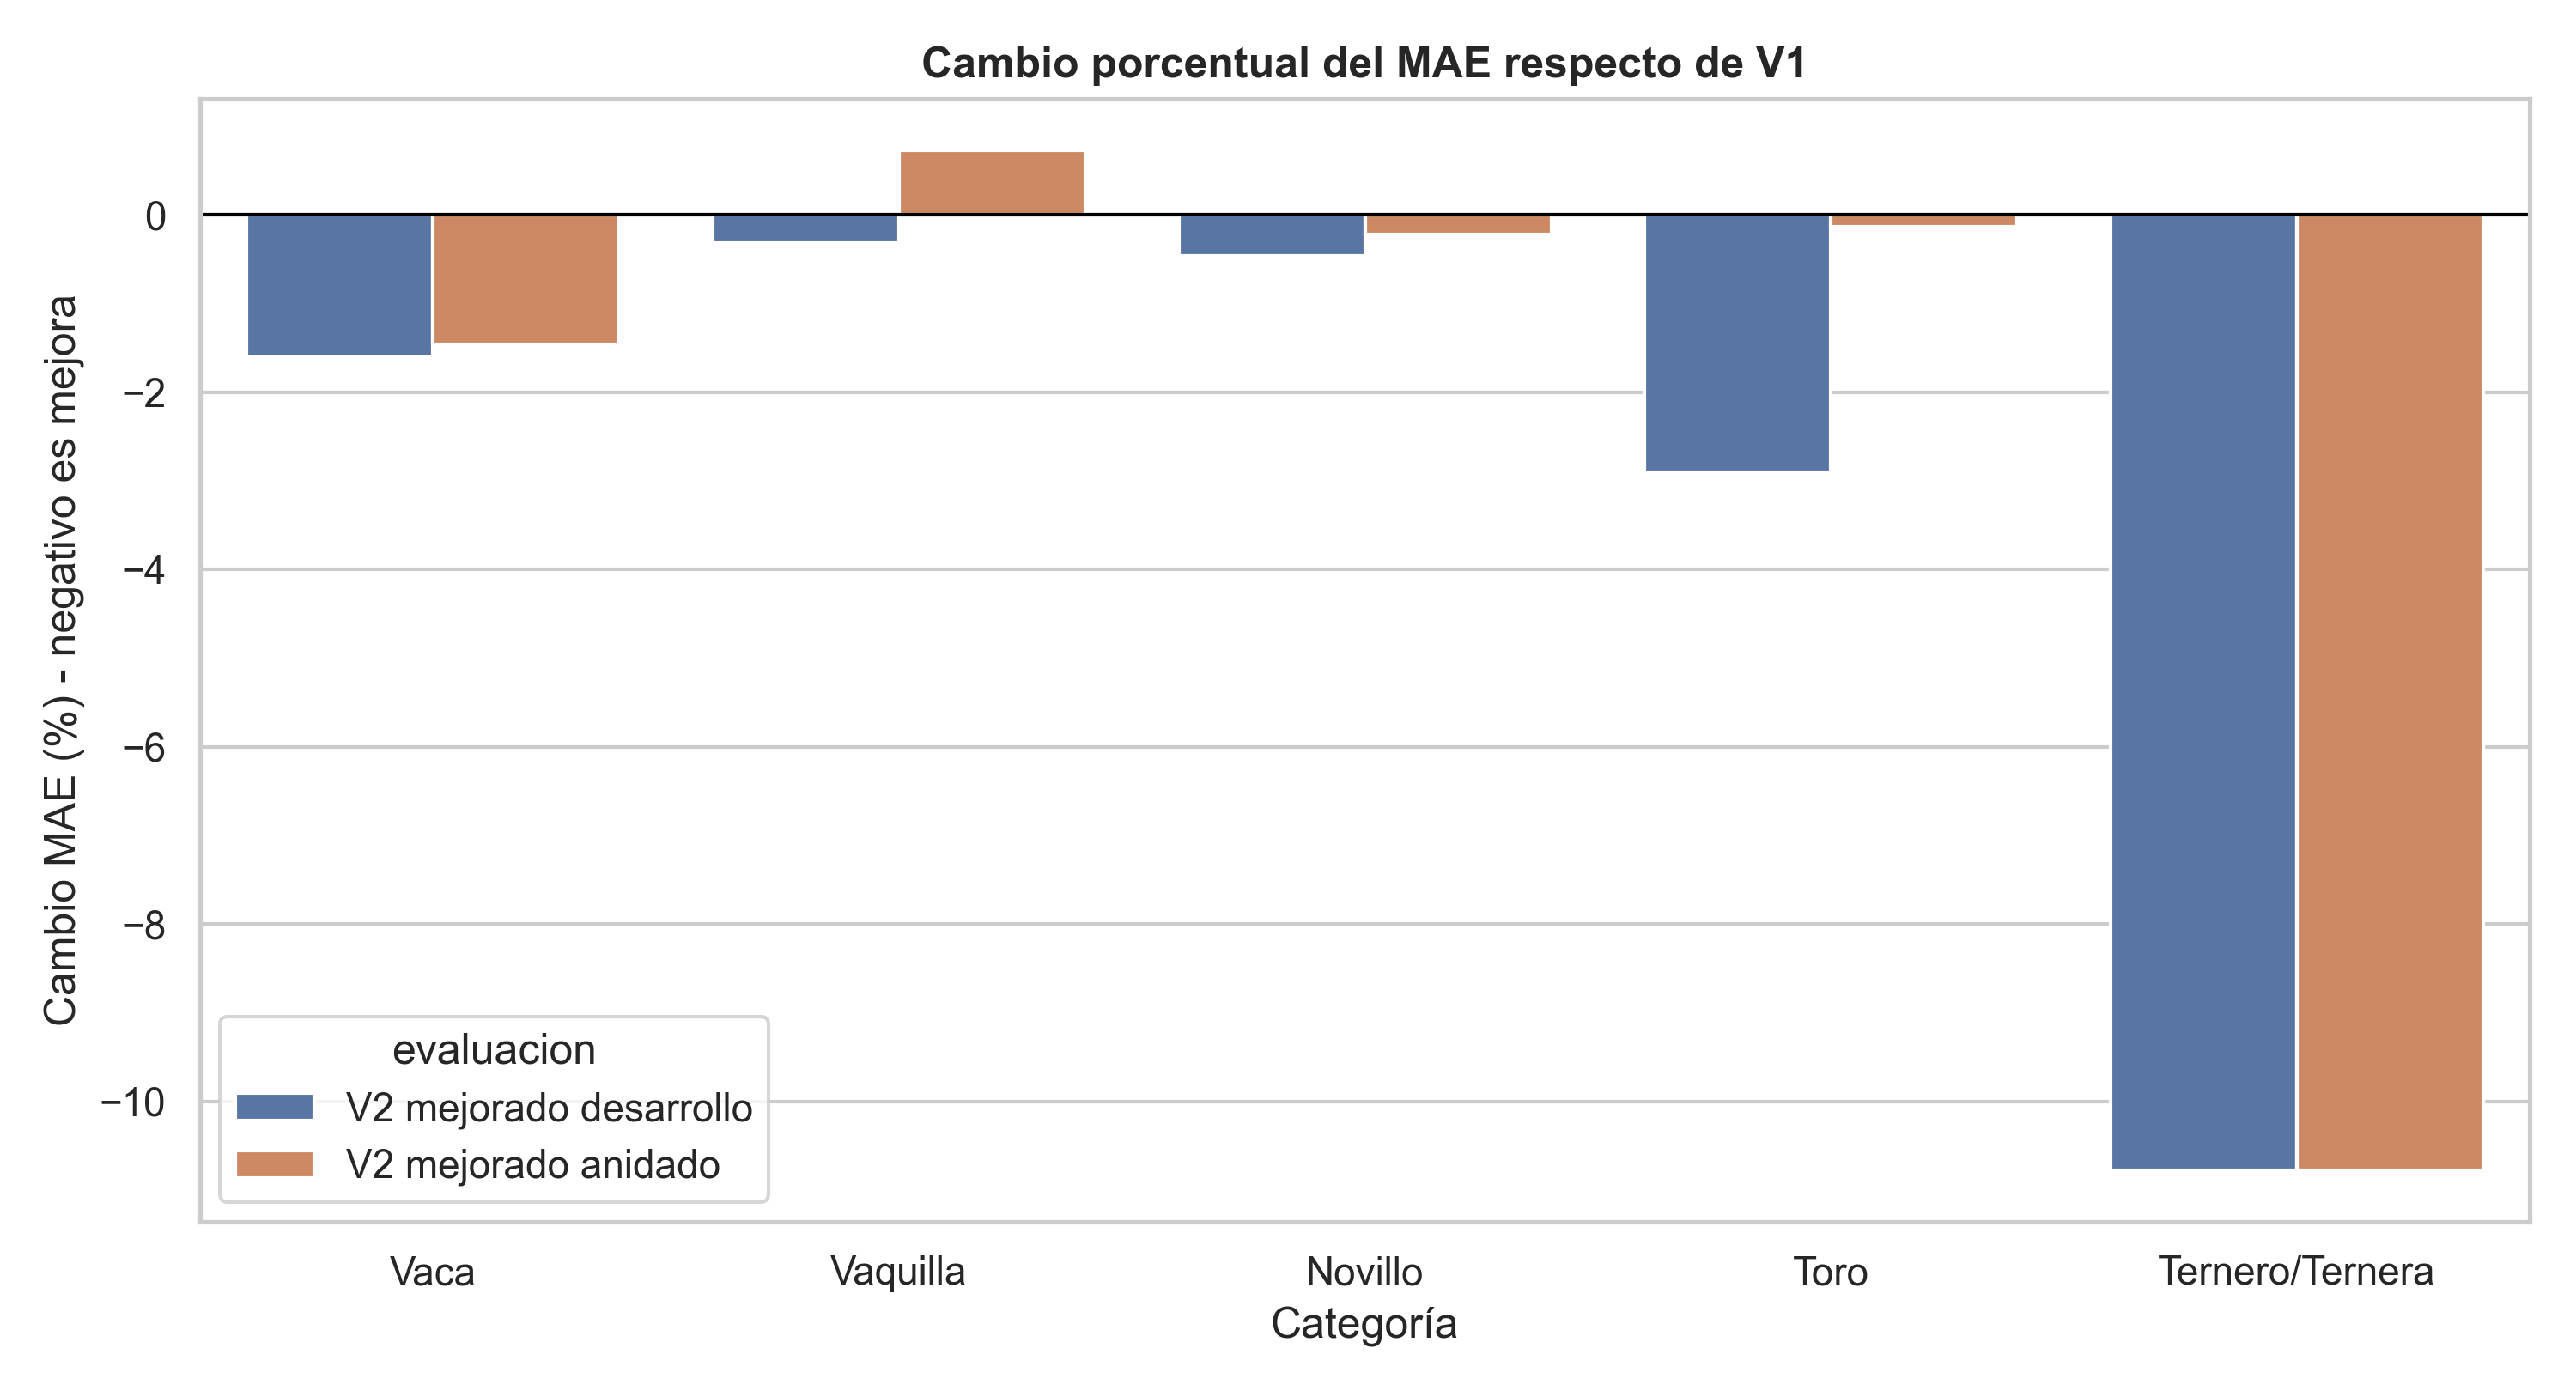
\includegraphics[width=0.94\textwidth]{figures_metricas_detalladas/6_cambio_porcentual_mae.png}
\caption{Cambio porcentual del MAE respecto de V1. Los valores negativos representan mejora.}
\end{figure}

\subsection{Comparación por fold}

\begin{figure}[H]
\centering
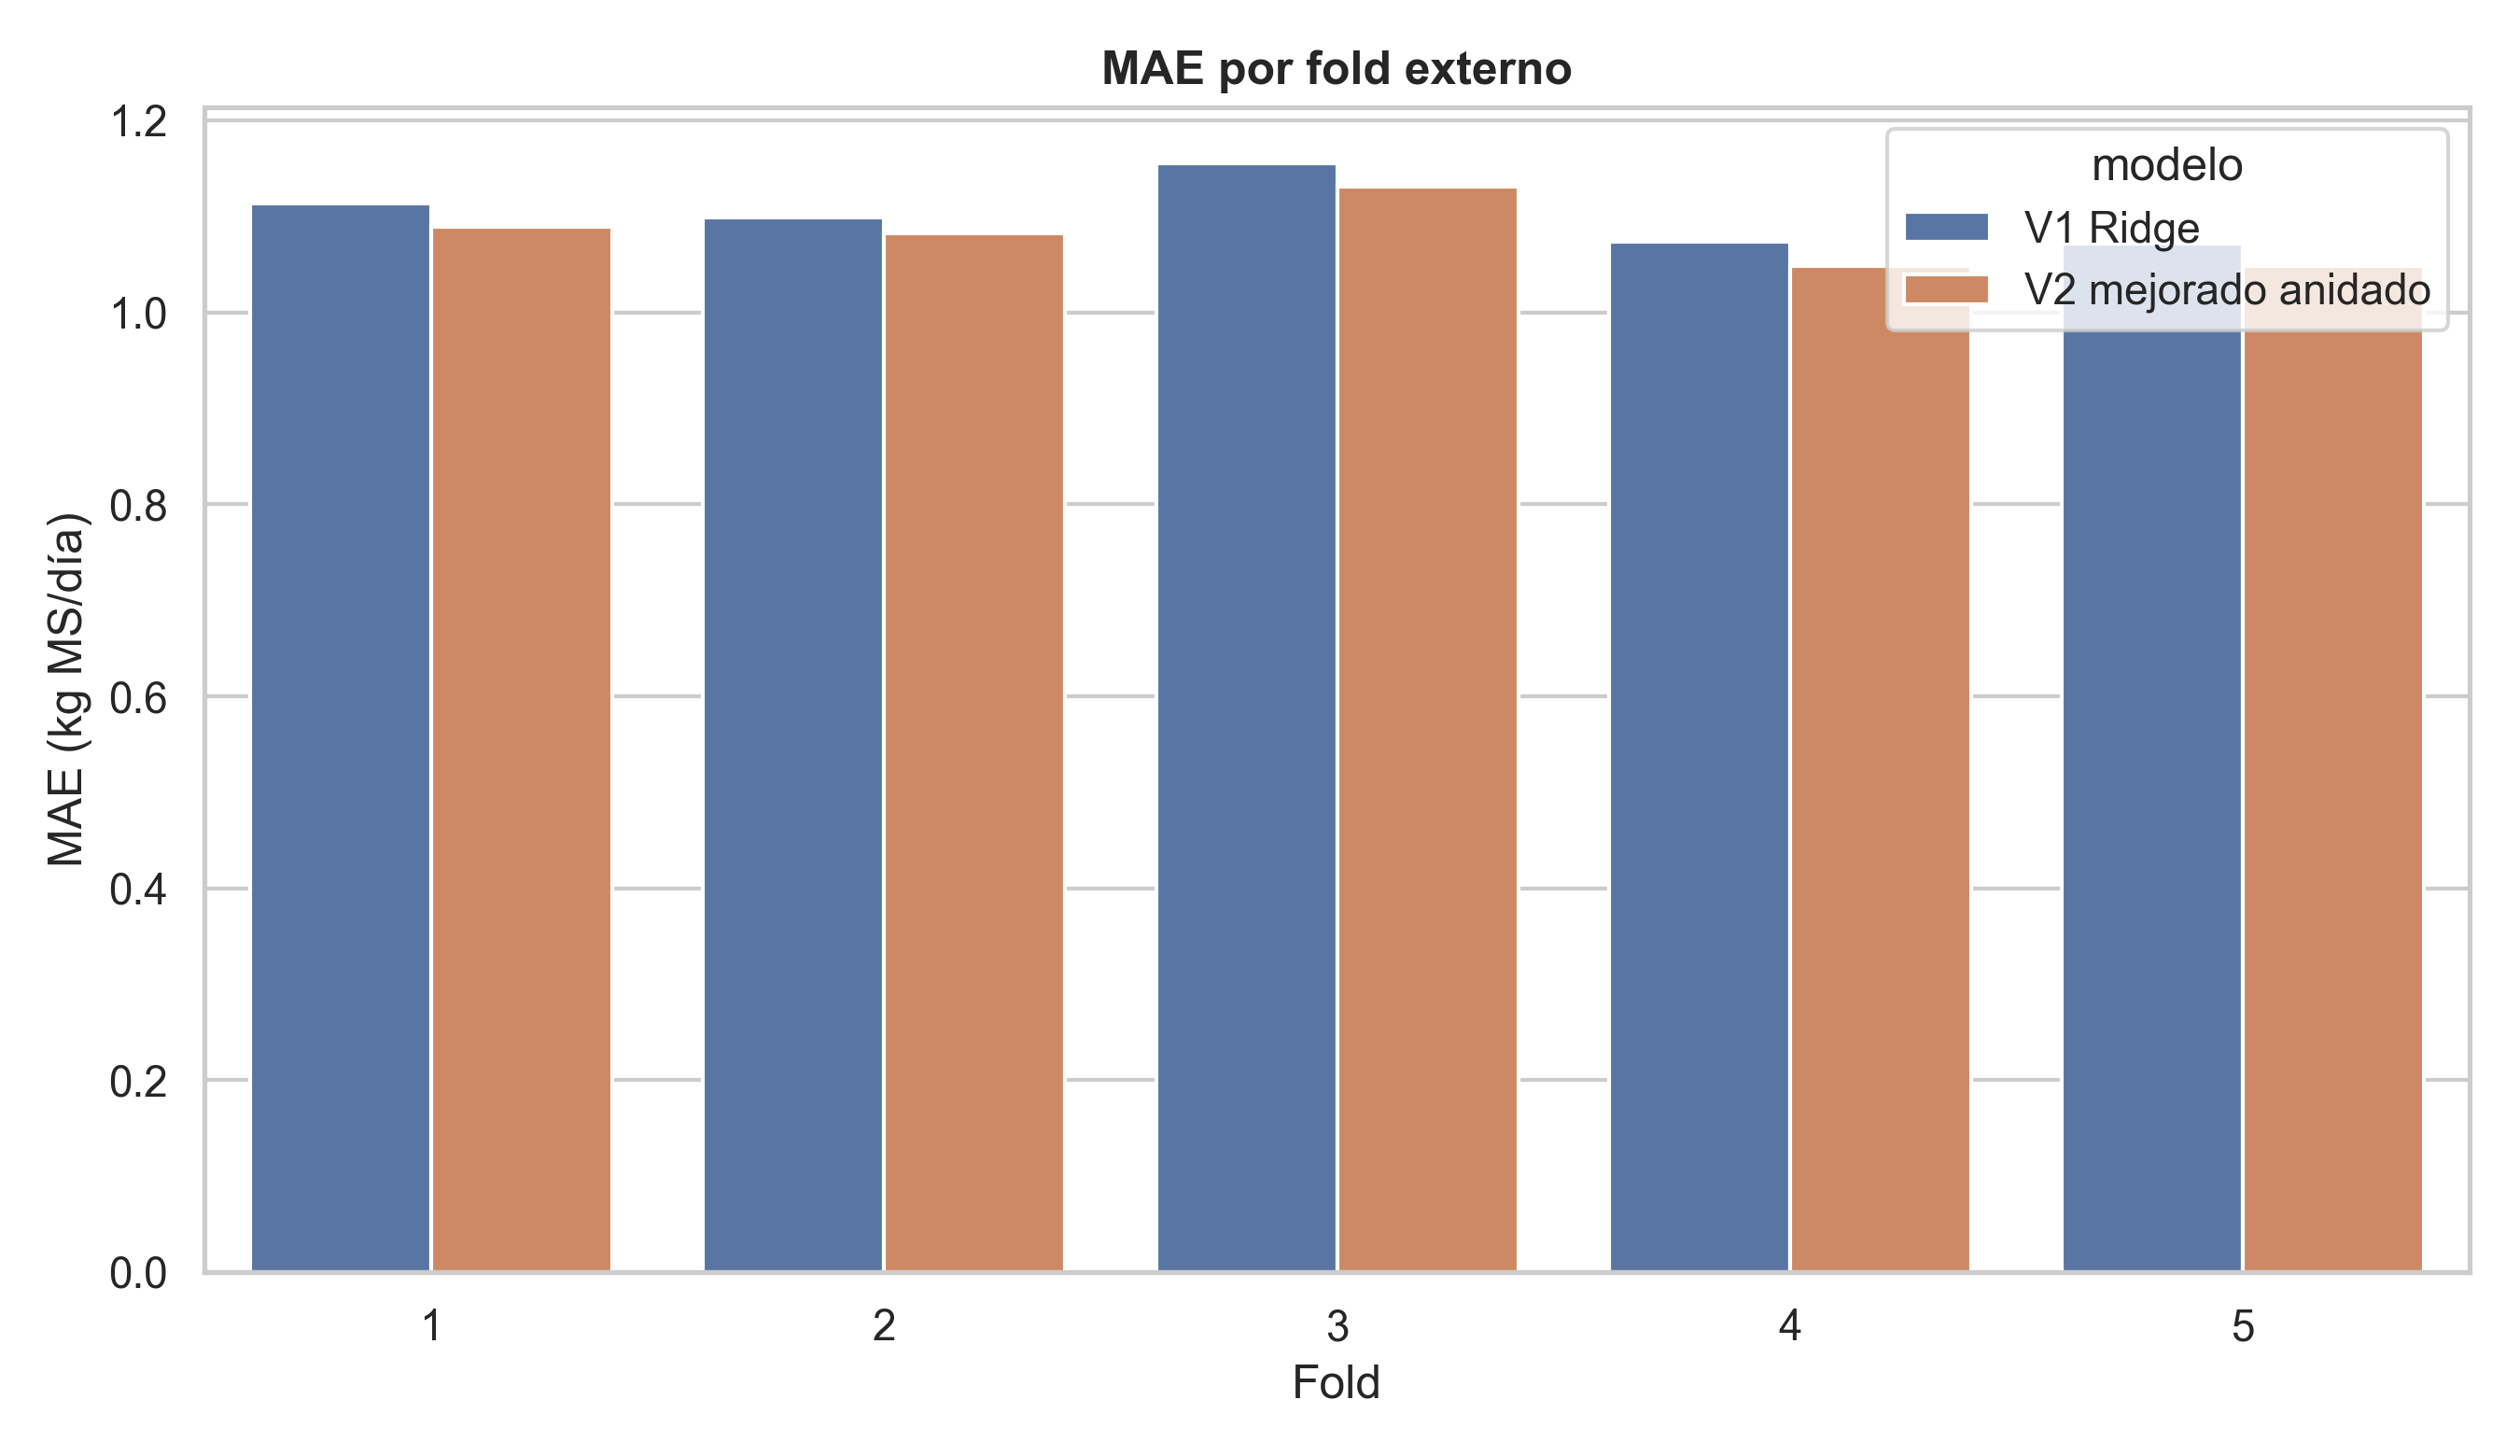
\includegraphics[width=0.9\textwidth]{figures_metricas_detalladas/5_mae_por_fold.png}
\caption{MAE por fold. Las comparaciones fold a fold deben interpretarse con cautela porque V2 mejorado realiza selección interna adicional.}
\end{figure}

V2 mejorado tiene menor MAE en los folds 1, 2, 3, 4 y 5 al comparar los valores reportados, aunque el tamaño de la ventaja cambia. Ambos modelos encuentran su mayor MAE en el fold 3 y uno de sus mejores resultados en los folds finales.

\subsection{¿Con qué modelo quedarse?}

Si la prioridad exclusiva es el rendimiento predictivo observado, se recomienda \textbf{V2 mejorado}. Obtiene mejor MAE, RMSE y $R^2$ globales bajo la evaluación anidada y la ventaja principal se mantiene sin utilizar el fold externo para seleccionar la configuración.

Si la prioridad es simplicidad, auditabilidad, velocidad y facilidad de mantenimiento, \textbf{V1 Ridge} sigue siendo una elección defendible. La mejora global de V2 mejorado no es grande y no aparece en todas las categorías.

La decisión práctica es conservar ambos artefactos: V2 mejorado como mejor alternativa experimental y V1 como referencia estable y respaldo.

\section{Inferencia y uso}

Los modelos finales están serializados en:
\begin{itemize}
  \item \codigo{models/dmi_model.joblib}: V1 Ridge;
  \item \codigo{models/dmi_model_v2_mejorado.joblib}: ensamble mejorado.
\end{itemize}

La clase \codigo{HerdPredictor} recibe lotes de animales, prepara las mismas cuatro entradas usadas durante el entrenamiento y devuelve DMI absoluto y porcentaje del peso vivo. También compara el peso con el rango histórico de la categoría para advertir extrapolaciones.

\begin{table}[H]
\centering
\caption{Rangos de peso observados durante el entrenamiento.}
\begin{tabular}{lrr}
\toprule
\textbf{Categoría} & \textbf{Mínimo (kg)} & \textbf{Máximo (kg)}\\
\midrule
Vaca & 79,1 & 525,2\\
Vaquilla & 54,6 & 412,8\\
Novillo & 59,5 & 278,9\\
Toro & 97,0 & 595,5\\
Ternero/Ternera & 19,6 & 235,9\\
\bottomrule
\end{tabular}
\end{table}

Una predicción fuera de esos rangos no es necesariamente imposible, pero implica extrapolación. Tampoco debe interpretarse una estimación puntual como una prescripción exacta ni como sustituto de criterio profesional.

\section{Limitaciones y validez}

\begin{itemize}
  \item Los datos proceden de Bomet, Kenia; no existe validación externa en otra región.
  \item No se incluyen clima, raza, edad exacta, calidad o disponibilidad de forraje, dieta, producción láctea ni manejo.
  \item Existen mediciones repetidas por animal; el agrupamiento se realiza por hogar, no por identificador animal y hogar simultáneamente.
  \item Hay 1.421 filas con \codigo{id_ambiguo}; no se dispone de análisis de sensibilidad excluyéndolas.
  \item El CSV crudo original y la transformación histórica no están disponibles.
  \item Los estados fisiológicos combinados tienen muy pocas observaciones.
  \item No hay conjunto de prueba externo, intervalos predictivos ni evaluación prospectiva.
  \item La mejora de V2 mejorado es globalmente pequeña y heterogénea por categoría.
\end{itemize}

Las métricas demuestran generalización entre hogares del mismo dataset bajo el diseño utilizado. No demuestran automáticamente validez para decisiones nutricionales en otros países, sistemas productivos o condiciones ambientales.

\section{Conclusiones}

El proyecto construyó un flujo reproducible para estimar el consumo diario de materia seca con cuatro variables disponibles por animal. El dataset contiene señal predictiva clara: V1 Ridge reduce aproximadamente 48,2\% el MAE frente a predecir la media y explica alrededor del 68\% de la variabilidad bajo su validación interna.

V1 ofrece una base sólida, pequeña y transparente. Su principal debilidad es imponer una relación global a categorías heterogéneas. V2 mejorado responde a esa limitación mediante un ensamble que conserva Ridge y agrega especialistas validados por categoría.

La validación anidada favorece V2 mejorado: MAE 1,0791 frente a 1,1019; RMSE 1,5332 frente a 1,5354; y $R^2=0,6830$ frente a 0,6821. La reducción global de MAE es aproximadamente 2,07\%. La ganancia más importante corresponde a Ternero/Ternera, mientras Vaquilla empeora levemente y Toro muestra una combinación de MAE similar con peor RMSE y $R^2$.

Por resultados se elige \textbf{V2 mejorado}, pero la conclusión debe formularse con prudencia: es una mejora moderada, no una superioridad amplia. Antes de utilizarlo en producción se recomienda validar con datos externos y locales, documentar la fuente original, incorporar variables nutricionales y ambientales, estudiar los identificadores ambiguos y estimar incertidumbre de cada predicción.

\end{document}
